% options:
% thesis=B bachelor's thesis
% thesis=M master's thesis
% czech thesis in Czech language
% english thesis in English language
% hidelinks remove colour boxes around hyperlinks

\documentclass[thesis=M,czech]{FITthesis}[2012/10/20]

 \usepackage[utf8]{inputenc} % LaTeX source encoded as UTF-8
% \usepackage[latin2]{inputenc} % LaTeX source encoded as ISO-8859-2
% \usepackage[cp1250]{inputenc} % LaTeX source encoded as Windows-1250

\usepackage{graphicx} %graphics files inclusion
% \usepackage{subfig} %subfigures
% \usepackage{amsmath} %advanced maths
% \usepackage{amssymb} %additional math symbols

\usepackage{dirtree} %directory tree visualisation
\usepackage{svg}
\usepackage{amsmath}
\usepackage{url}
\usepackage{amsfonts}
\usepackage{multirow}
\usepackage{listings}

% % list of acronyms
% \usepackage[acronym,nonumberlist,toc,numberedsection=autolabel]{glossaries}
% \iflanguage{czech}{\renewcommand*{\acronymname}{Seznam pou{\v z}it{\' y}ch zkratek}}{}
% \makeglossaries


\setlength{\fboxsep}{0.005pt}
\newcommand{\tmpframe}[1]{\fbox{#1}}
%\renewcommand{\tmpframe}[1]{#1}

% setting out our listings to be nice
\lstset{basicstyle=\footnotesize\ttfamily,breaklines=true,showstringspaces=false,captionpos=b}
\renewcommand{\lstlistingname}{Kód}

% % % % % % % % % % % % % % % % % % % % % % % % % % % % % % 
% EDIT THIS
% % % % % % % % % % % % % % % % % % % % % % % % % % % % % % 

\department{Department of Katedra teoretické informatiky}
\title{Analýza bezpečnostních rizik aplikací z logů v reálném čase}
\authorGN{Vojtěch} %author's given name/names
\authorFN{Krákora} %author's surname
\author{Vojtěch Krákora} %author's name without academic degrees
\authorWithDegrees{Bc. Vojtěch Krákora} %author's name with academic degrees
\supervisor{Pavel Pivoňka, GWCPM}
\acknowledgements{THANKS (remove entirely in case you do not with to thank anyone)}
\abstractEN{Summarize the contents and contribution of your work in a few sentences in English language.}
\abstractCS{V n{\v e}kolika v{\v e}t{\' a}ch shr{\v n}te obsah a p{\v r}{\' i}nos t{\' e}to pr{\' a}ce v {\v c}esk{\' e}m jazyce.}
\placeForDeclarationOfAuthenticity{Prague}
\keywordsCS{Replace with comma-separated list of keywords in Czech.}
\keywordsEN{Replace with comma-separated list of keywords in English.}
\declarationOfAuthenticityOption{1} %select as appropriate, according to the desired license (integer 1-6)
% \website{http://site.example/thesis} %optional thesis URL


\usepackage{xcolor} 
\newcommand{\todo}[1]{\textcolor{red}{\textbf{[[#1]]}}}

\usepackage{blindtext}
\newcommand{\blind}[1][1]{\textcolor{gray}{\Blindtext[#1][1]}}



\begin{document}

% \newacronym{CVUT}{{\v C}VUT}{{\v C}esk{\' e} vysok{\' e} u{\v c}en{\' i} technick{\' e} v Praze}
% \newacronym{FIT}{FIT}{Fakulta informa{\v c}n{\' i}ch technologi{\' i}}

\setsecnumdepth{part}
\chapter{Introduction}
\todo{Napsat max jednu stranku}
S roustoucím významem informačních systémů a informací jenž jsou zpracovány počítaočovými systémy je kladen důraz na zabezpečení informací. Bezpečnost informačních systémů je zajišťována zákonem o kybernetické bezpečnosti 181/2014 Sb \cite{zakon181-2014}. Mnoho systémů vyžaduje i vyšší zabezpečení například pomocí ISO normy 27001 \cite{iso27001}.

\blind[2]


\setsecnumdepth{all}
\chapter{Úvod do problematiky}
	
	
	\section{Kybernetická bezpečnost}
		Pro dnešní dobu je běžné využívání informačních technologií prakticky kdekoliv. Jde o stavební kámen mnoha podniků. Informačním systémem rozumíme kombinaci softwaru, hardwaru, infrastruktury a trénovaného personálu \cite{businessdictionary} .  Tam, kde  se informační systémy vyskytují pomáhají práci zjednodušovat, tvořit, či se jinak podílet. Systémy je třeba udržovat v provozu a co nejvíce se vyhnout všem možným rizikům, které mohou narušit obchodní proces.
		
		Obecně lze na zabezpečení informačního systému nahlížet z mnoha různých úhlů. Zabezpečit lze síť pomocí certifikovaného přístupu, správně zabezpečené bezdrátové sítě. Do operačních systémů se nainstalují antivirové programy. Samotná zařízení se fyzicky uzamknou a znemožní se přístup nepovolaným osobám  a podobně.
		
		Povinnost zabezpečovat informační systémy přikládá zákon o kybernetické bezpečnosti 181/2014 Sb. Tento zákon stanovuje povinnosti a práva orgánů veřejné moci v oblasti kybernetické bezpečnosti \cite{zakon181-2014}. Tento zákon mimo jiné nařizuje orgánům veřejné moci povinnost zajišťovat kybernetickou bezpečnost.
		
		Kromě zákonu jsou k dispozici normy. Jednou z takových norem je norma ISO 27001. Tato norma stanovuje požadavky, které je nutné dodržovat pro kybernetickou bezpečnost. Tyto požadavky jsou stanoveny jak na samotné informační systémy, tak i na zaměstnance, informační procesy, či strategie firmy. \cite{iso27001}.
		
		Lze říci, že zajištění kybernetické bezpečnosti a následné detekci jednotlivých bezpečnostních rizik je velmi specifické. Každá určitá doména má svá rizika a jiné druhy způsobů jejich detekce. 
		
		V práci řeším kybernetickou bezpečnost pro konkrétní část informačního systému. Podstatná tedy jsou bezpečností rizika na integrační platformě Unify. Definice integrační platformy a její popis je v sekci \ref{sec:unify}.
		
		\subsection{Bezpečnostní rizika}
		\todo{Nadefinovat bezpečnostní rizika}
			Jak již bylo uvedeno pro tuto práci jsou podstatná bezpečností rizika na konkrétní integrační platformě. Cílem je hledat pouze ta, která vznikají na straně programu. Zabezpečení přístupů fyzicky k serverům Unify a podobně nebudou probírána.
			
			\subsubsection{Zero day útoky}
				\label{sec:zero-day}
				Zero day útoky lze volně přeložit jako útoky nultého dne.
				Jde o taková bezpečnostní rizika, která využívají zranitelností nějakého systému, nebo jeho části, která nebyla zveřejněna \cite{investigationZ0}.
				
				Integrační platforma je složena z mnoha modulů, který tvoří její celek. S rostoucím množstvím softwaru a použitých knihoven jsou šance na skrytou chybu velmi vysoké. 
			
			\subsubsection{Odepření služby}
				Útoky, jenž se snaží o znemožnění užívání nějaké služby jejími uživateli označujeme jako DoS. Zkratka DoS \todo{Zkratka DoS} pochází z anglického názvu \textit{Denial of service}, přeloženo jako odepření služby. Poddruhem DoS útoku je DDoS (z anglického \textit{distributed denial of service}). Při DDoS je použito velké množství různých zařízení, které požadovanou službu zahltí požadavky. Cílem je, aby služba nedokázala požadavky odbavovat a došlo tím k tomu, aby nové požadavky odmítala \cite{dosAndDdos}.
				
				Ukázka rozdílu mezi DoS a DDoS je na obrázku \ref{fig:ddos}. V části s DoS je znázorněn útočník, který se snaží znepřístupnit službu. U DDoS útočník využije nakažené PC \todo{zkratka PC} ( obecně to mohou být i mobilní telefony, tablety, či jiná zařízení s přístupem do sítě) a následně jejich pomocí zahlcuje cílovou službu.	
				
				\begin{figure}[htb]\centering
					\tmpframe{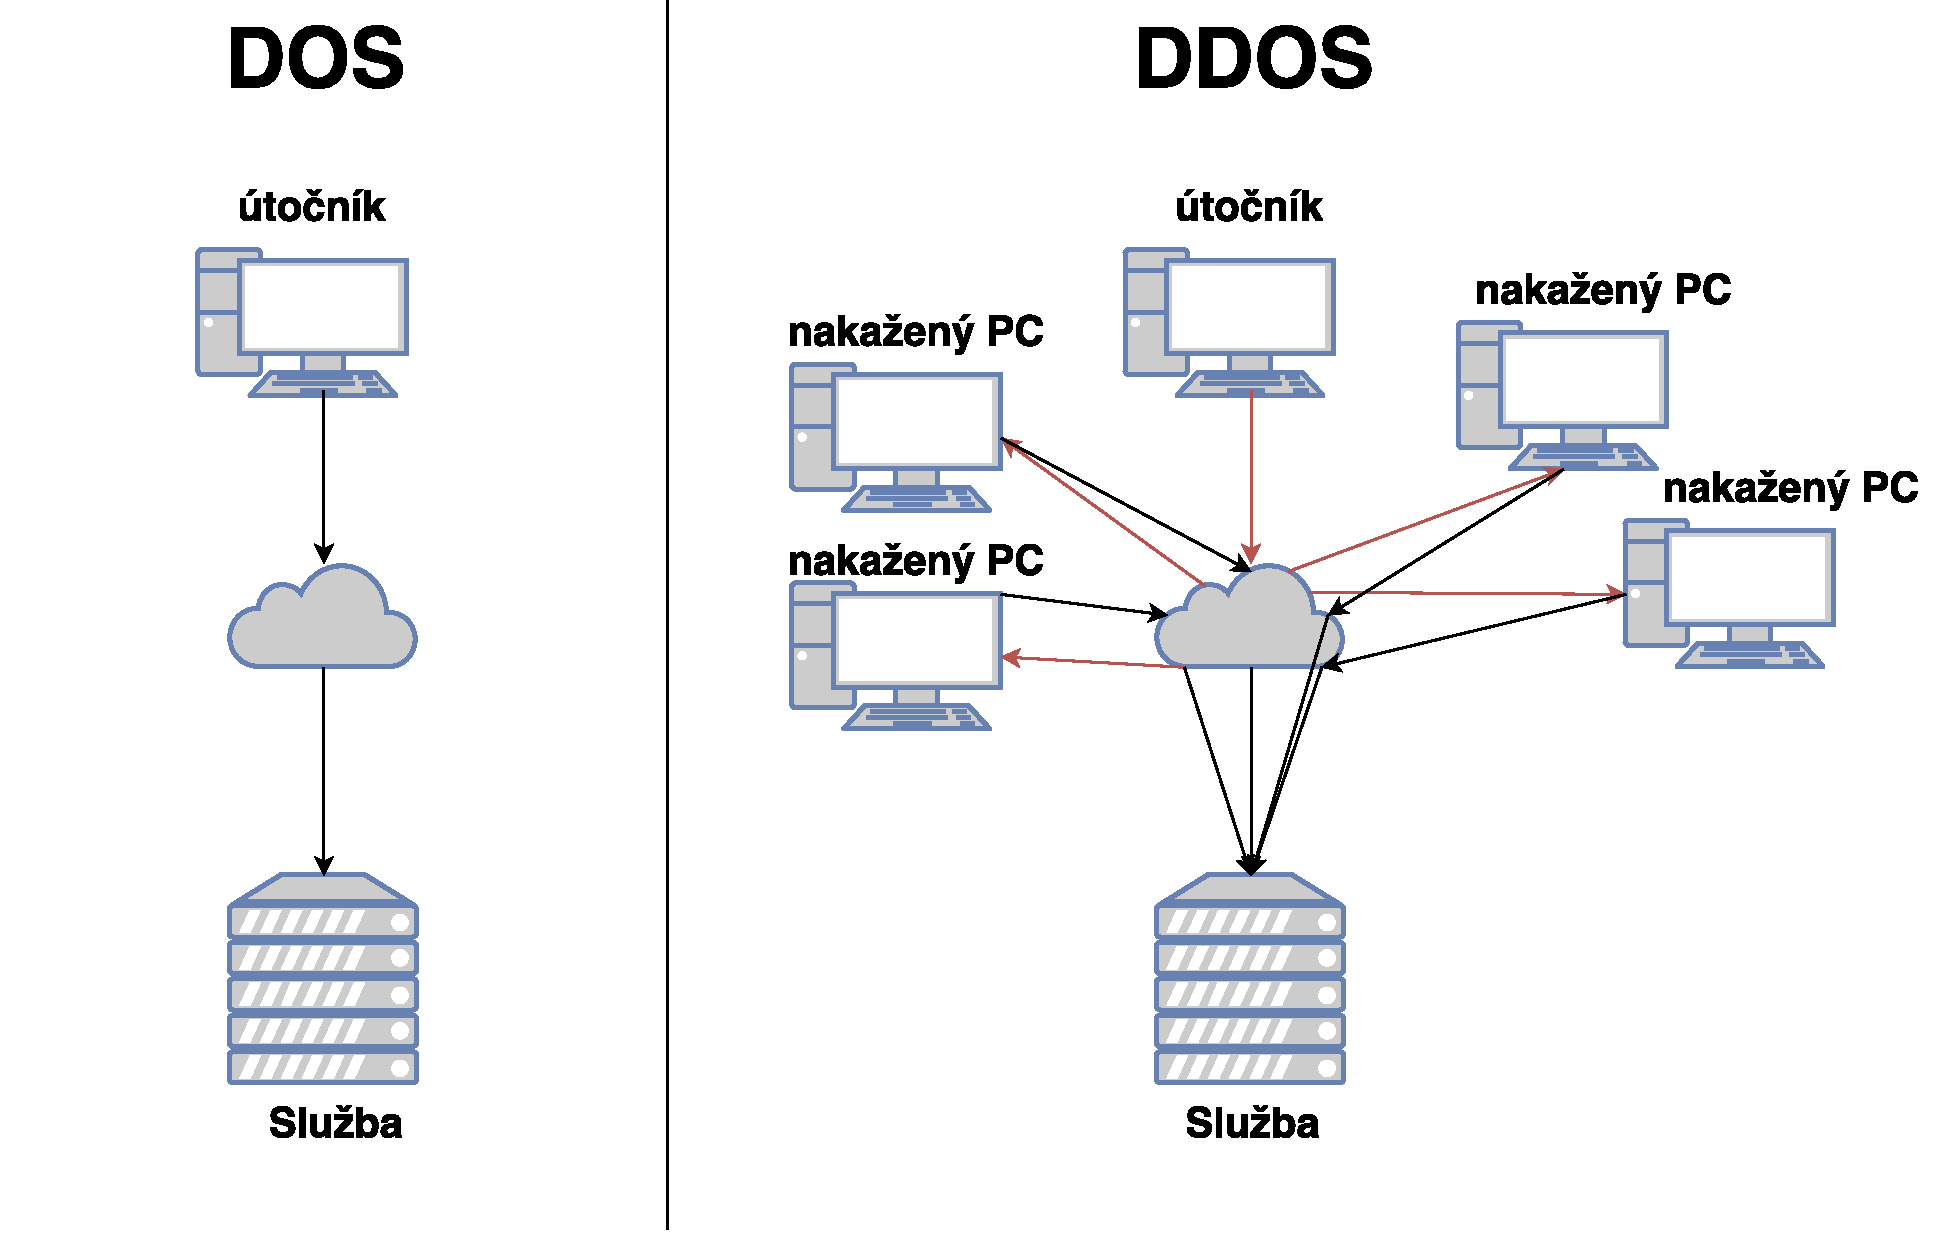
\includegraphics[width=\textwidth]{./img/ddos}}		
					\caption{Grafické porovnání DoS a DDoS útoku.}
					\label{fig:ddos}
				\end{figure}
				
				Důsledky útoku se následně dotýkají mnoha uživatelů nedostupně služby. Proto je nutné nejen detekovat velké množství požadavků na vlastní služby, ale také například nedostupnost partnera, na jehož službu jsem připojen. Při včasné detekci je možné zjistit, že je partner pod DDoS útokem dříve, než to zjistí on. 
				
			    Jeden DDoS útok se odehrál na služby O2 v roce 2016. Jeho důsledky následně omezil i provoz integrační platformy, pro kterou je tato práce tvořena. 
			    \todo{DDOS na O2}
			
			\subsubsection{Nevalidní dotazy}
				Riziko, které je třeba hlídat, ale není nutně vytvořené za účelem poškodit někoho nebo něco. Integrační platforma musí zpracovávat různé požadavky od konzumentů a ty zpravidla přeposílat poskytovatelům služeb. Mohou nastat situace, kdy konzument posílá nevalidní požadavek.
			
				V případě, že požadavky jsou v xml formě, lze definovat přesné znění zprávy. V případě, že je její validita narušena dochází k nekompatibilnímu dotazu na rozhraní poskytovatele. To může vyústit v nevyřízené a odmítnuté požadavky. Z této situace mohou vzniknout nechtěné útoky odepření služeb. V případě, že požadavek nebude zamítnut, možným důsledkem může být zisk nevalidních dat nebo dokonce i dat, která se ke konzumentovi neměla dostat.
			
				Tyto popřípadě i jiné neočekávané situace je třeba včas odhalit a řešit.
				
			\subsubsection{Ostatní}
				Mnoho bezpečnostních rizik může být neznámých. Nelze vše zaškatulkovat do obecných kategorií. Rizikem mohou být i služby, které po autorizaci nabízí různé možnosti získání dat, například pomocí výběru z databáze. Z těchto důvodů je vhodné nezaměřovat se na konkrétní kategorie rizik, ale snažit se rozpoznávat rizika jakožto celek.	
			
		\subsection{Zjišťování bezpečnostních rizik}
			Rozpoznávat bezpečnostní rizika je při jejich různorodosti složitý úkol. Základem je dodržovat bezpečnostní pravidla například při manipulaci s hesly. Na platformě, kde se lze setkat se stovkami služeb se bude vyskytovat velké množství hesel. Správa těchto hesel není snadným úkolem. Přesto by se nemělo stát, že i třeba na testovacím prostředí aplikace se budou hesla zasílat e-mailovou komunikací. Hesla budou totožná jako uživatelská jména nebo dokonce zabezpečení nebude existovat. 
			
			V následujících kapitolách jsou popsány různé metody, jak na softwarové úrovni detekovat co nejvíce možných bezpečnostních rizik.
			
			\subsubsection{Posouzení kódu}
				Posouzení kódu ( anglicky code review) je metoda kontroly kvality kódu. Programátor, který napsal nějaká kus komponenty dá svou část programu na kontrolu druhé osobě. Není přímo nutné, aby kontrolující osoba byla nadřízený. Kontrolující programátor hlídá kvalitu kódu a zároveň prověřuje jeho funkčnost. Tato metoda vede ke zkvalitnění dodávaného softwaru, ale je finančně i časově náročná \todo{cite}. Lze ovšem říci, že finanční i časová náročnost jsou diskutabilní. Lze se setkat s tím, že kód, který neprošel posouzením druhou osobou nebude fungovat a charakteristika chyby neumožní její snadnou detekci. Pokud by se tato chyba odhalila pomocí posouzení, mohl být čas naopak ušetřen. Další důvod pro ušetření času jsou nutné birokratické procesy, které jsou nutné pro opravení chyby (například vytvoření opravné dávky, manuálu a kontaktování release managementu). To už hodně záleží na procesech, které jsou při vývoji používány. 
			
			Zvýšením kontroly se i zvyšuje šance na detekci bezpečnostního rizika. Jako velmi efektivní metodu ji uvádí zdroj \cite{pethukovKozlovVulnerabilities}.
			
			\subsubsection{Analýza z pohledu uživatele}
				Ve snaze celý proces detekce bezpečnostních rizik zautomatizovat se používá i metoda založená na pohledu uživatele aplikace \cite{pethukovKozlovVulnerabilities}. Aplikace má své uživatele, proto je možné vytvářet scénáře, kdy se uživatel pokouší najít v aplikaci nějaký nedostatek. Takový nedostatek může následně produkovat bezpečnostní riziko. Automatizace těchto scénářů je zpravidla snadno proveditelná a často patří do klasických testovacích scénářů.
				
				Testují se například SQL injection, přístup do neoprávněných míst a další.
				
			\subsection{Analýza na straně serveru}
				Předchozí způsoby se snažili zabránit výskytu rizik. Pro zachování kybernetické bezpečnosti je vhodné sledovat i aktuální situaci v aplikaci. Vzhledem k rozsahu moderních aplikací je takřka vyloučené, že bychom dokázali rizikům předejít. Sledování aktuálního stavu a provozu můžeme být schopni detekovat podezřelé činnosti. Na základě toho pak dokážeme zjistit bezpečnostní riziko.
				
				I zde lze využit automatizaci. Například ve zdroji \cite{CoronaGiacintoDetWebAtt} je uveden systém na rozpoznání vzorů zpráv. Koncept založený na znalostním inženýrství může pomoci detekovat i využití zranitelnosti nultého dne (\ref{sec:zero-day}) \cite{AhnKimChungBigDataAnal}.
				
				Podobný princip využívají i systémy SIEM (security information and event management). SIEM se zabývá bezpečnostním management. Jeho myšlenka je taková, že  
				rozsáhlé aplikace mají své zdroje informací (logy) na různých místem, ale je zapotřebí k nim přistupovat z jednoho místa. Z tohoto místa se provádí následná analýza kompletně všech zdrojů a vyhodnocují se bezpečnostní rizika \cite{SIEMDef}. Pomocí tohoto vyhodnocení pak může specializovaný personál reagovat na vzniklou situaci. Grafické znázornění příkladu SIEM je na obrázku \ref{fig:siem}.
				
				\begin{figure}[htb]\centering
					\tmpframe{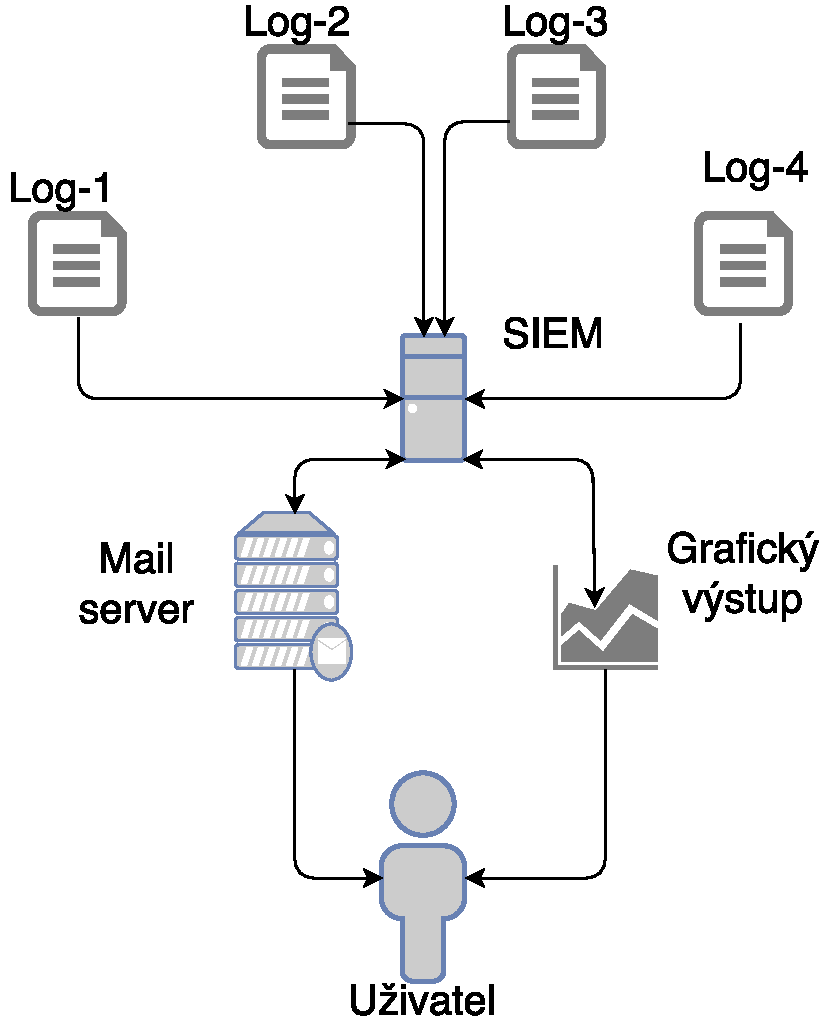
\includegraphics[scale=0.5]{./img/SIEM}}		
					\caption{Grafické znázornění SIEM.}
					\label{fig:siem}
				\end{figure}
			
	\section{Integrační platforma unify}
		\label{sec:unify}
		Jedním z cílů práce je detekovat bezpečnostní rizika na integrační platformě Unify \cite{unify}. Integrace je proces, který propojuje nesourodé systémy, tak aby umožnil jejich snadnou komunikaci \cite{integration}. 
		
		\subsection{Význam Unify}
			\label{sec:meaning-unify}
			Jak je uvedeno ve zdroji \cite{unify}, Unify pracuje se webovými službami, zprávami, transformací a směrováním dat nebo také přenosem souborů. Její význam koordinace interakcí mezi různými podnikovými systémy.
			
			Rozsáhlé systémy se skládají z odlišných komponent. Komponenty mohou být například databázové, webové nebo souborové. Aby se zajistila komunikace mezi nimi, je vytvářena integrační platforma. Základem Unify je sběrnice ESB (enterprise service bus). Tato sběrnice vystavuje různé interfacy a je schopna volat veškeré nutné komponenty. Jednotlivé komponenty pak nekomunikují mezi sebou napřímo, ale skrz ESB. 
			
			Podobný přístup je i pro partnery mimo domovskou organizaci, kde je Unify provozováno. Každý takový partner je připojen na B2B sběrnici (business to business). Ta stejně jako ESB vystavuje interfacy a následně volá rozhraní ESB. Význam B2B je takový, že se zpravidla vyskytuje takzvaně demilitarizované zóně. Z tohoto důvodu je nutné zde dbát na vyšší bezpečnost provozu.
			
			Mimo zmíněných sběrnic je Unify složeno i z dalších komponent. Například notifikační engine slouží k rozesílání mailových nebo po připojení na SMS konektor i SMS zpráv \todo{Zkratka SMS}. Komponenta ETL (extract transform load) zpravidla transformuje data z jednoho uložiště do druhého. SFE (secure file exchange) má za úkol přenos souborů. Tento přenos se hlavně využívá mezi demilitarizovanou zónou a vnitřní sítí.
			
		\subsection{Technologie}
			\label{sec:unify-technologi}
			Unify je postaveno na otevřeném softwaru. Hlavní použité technologie jsou: 
			
			\begin{itemize} 
				\item \textbf{JBoss} - aplikační server s podporou Java EE 6 \cite{oracleJavaEE6}
				\item \textbf{Switchyard} - vývojářský framework, který pomocí Apache Camel\texttrademark  umožňuje snažší vývoj aplikací postupy architektury orientované na služby 
				\item \textbf{Apache Camel \texttrademark } - otevřený software jakožto aplikační rámec pro integraci
				\item \textbf{Databáze} - pro účel přeposílání zpráv a journalování zpráv se využívají databáze
				\item \textbf{Nginx SW Load balancer} - webový servere, který distribuuje zprávy mezi dva, či více totožných serverů za účelem rozložení zátěže   		
			\end{itemize}
			
			
		\subsection{Architektura Unify}
			Architektura již byla z části popsána v sekci \ref{sec:meaning-unify}. Skládá se tedy ze dvou sběrnic, kde jedna slouží pro komunikaci vnitřních systémů a druhá pro komunikaci se systémy partnerů. Dále Unify obsahuje různé komponenty pro prací s daty nebo jejich přenos, popřípadě rozesílání emailů a sms zpráv.
			Architekturu přibližuje obrázek \ref{fig:esb}. 
			
			\begin{figure}[htb]\centering
				\tmpframe{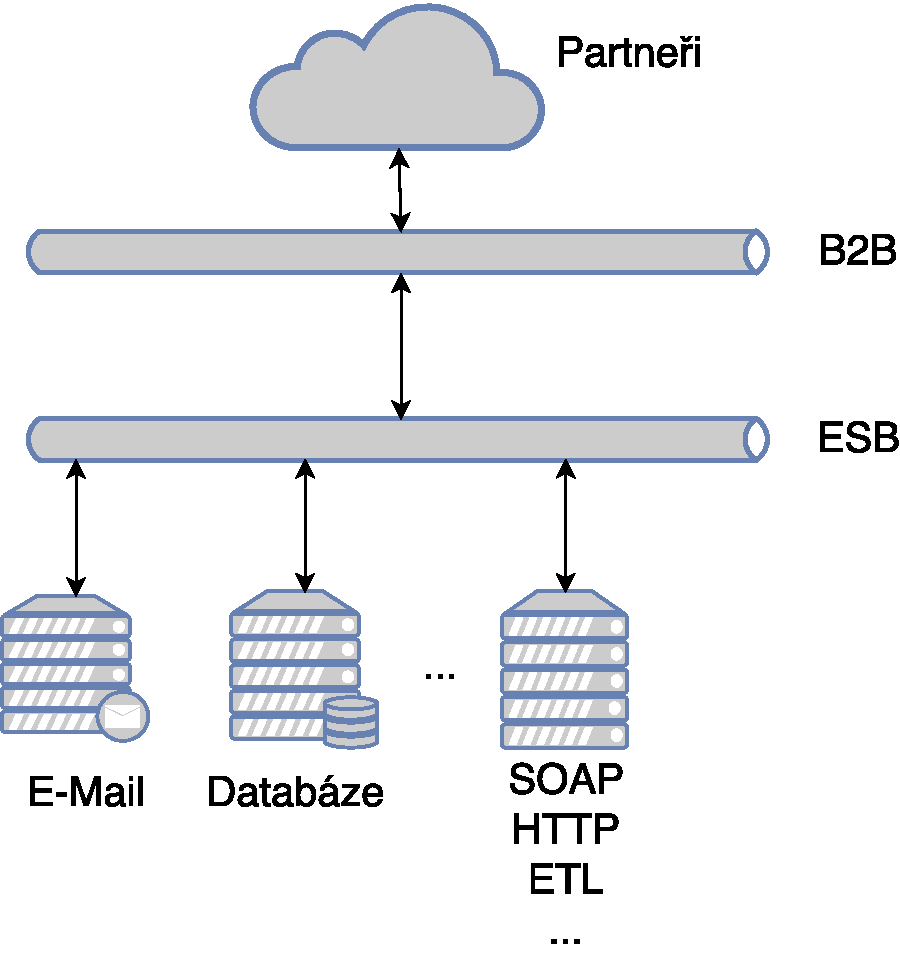
\includegraphics[scale=0.5]{./img/Unify-Easy}}		
				\caption{Enterprise Service Bus.}
				\label{fig:esb}
			\end{figure}
		
			Mimo sběrnic a komponent Unify obsahuje i uživatelské rozhraní, sloužící pro konfiguraci. 
			
			Z použitých technologí v kapitole \ref{sec:unify-technologi} plyne, že hlavním stavebním kamenem pro implementaci je Java EE 6.
		
		\todo{Zkratky B2B,ESB}
		
		\subsection{Komunikace na Unify}
			Jak bylo zmíněno, na Unify je komunikace jak pomocí XML zpráv, JSON zpráv, tak například i přenosem souborů. Největší provoz je zpravidla na sběrnici ESB. Požadavky na ESB lze rozdělit na tři druhy:
			
			\subsubsection{Synchronní zprávy}
				Konzument odešle požadavek, na který okamžitě dostane odpověď o tom, zdali se ho podařilo doručit. Doručení nezajišťuje i zpracování požadavku cílovým systémem. Byť u časově nenáročných požadavků je i to možné. Využití je zpravidla na dotazující se služby. Kdy synchronně na zprávu dostaneme odpověď s informací na kterou jsme se tázali. V obrázku \ref{fig:esb_communication} část \uv{A)}.
			
			\subsubsection{Asynchronní zprávy}
				Asynchronní zprávy se na Unify dají rozdělit na dvě synchronní. První je dotaz konzumenta služby, na který obdrží okamžitou odpověď o přijetí požadavku. Jakmile je požadavek cílovým systémem zpracován, je odeslána zpět konzumentovi synchronní zpráva, která informuje i o zpracování požadavku. Běžné využití je pro takové služby, které požadavek zpracovávají delší dobu. V obrázku \ref{fig:esb_communication} část \uv{B)}.
			
			\subsubsection{Zprávy s frontou}
				Je-li nutné mít jistotu odeslání požadavku (zpravidla například nové objednávky) pošle se dotaz na službu s frontou. Služba si požadavek uloží do fronty a odpoví zpět konzumentovi informací o přijetí. Následně požadavek odešle cílovému systému. Jakmile od systémy obdrží kladnou synchronní odpověď o zpracování vyjme požadavek z fronty a více ho nevolá. V opačném případě zkusí požadavek poslat po nějaké době znova. V obrázku \ref{fig:esb_communication} část \uv{C)}.
				
				\begin{figure}[htb]\centering
					\tmpframe{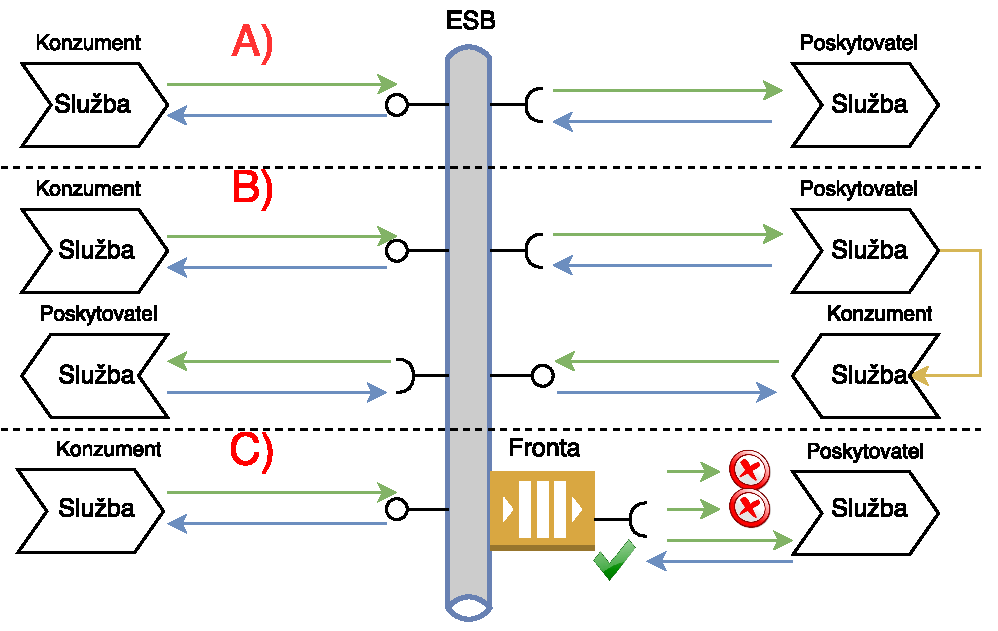
\includegraphics[width=\textwidth]{./img/basic_esb_communication}}		
					\caption{Běžné druhy komunikace na ESB, Unify - A) Synchronní, B) Asynchronní C) Zprávy s frontou}
					\label{fig:esb_communication}
				\end{figure}
	
	\section{Strojové učení}
		Strojové učení patří jako jedna podkapitola do znalostního inženýrství. Jde o algoritmy a metody, které pomáhají stroji, aby se učil. Učením je myšleno, kdy stroj je schopen na základě zkušenosti se rozhodovat. Toto rozhodování dokáže vyvodit automaticky bez pomoci člověka. \cite{what-is-machine-learning}
		
		Strojové učení využíváno například ve spamových filtrech, v algoritmech rozpoznávajících obličej nebo jako automatické třídění článků.
		
		Základem jsou tři techniky:
		
			\begin{itemize} 
				\item učení s učitelem - algoritmus má na vstupu učící množinu dat a validační množinu
				\item učení bez učitele - algoritmus získá na vstupu pouze neoznačená vstupní data
				\item zpětnovazebné učení - algoritmus se učí pomocí zpětné vazby	
			\end{itemize}
		
		Zmíněné techniky se snaží implementovat jeden ze základních úkolů strojového učení:
			\begin{itemize} 
				\item klasifikace - rozdělení dat do konkrétních skupin
				\item regrese - nalezení správných hodnot pro vstupní data
				\item shlukování - rozdělení dat do skupin vzhledem k jejich vzájemné podobnosti
			\end{itemize}
		
		
		\todo{Zadnej zazrak} \cite{machine-learning}
		\todo{Obecny zacatek} \cite{machin-learning-and-opt}
		
	\subsection{Těžení textu}
		V logách integrační platformy je veškerá komunikace v textovém formátu. Kromě zpráv ve formátu XML jsou zde i zprávy ve formátu JSON, popřípadě výpisy chyb, pokud nějaká nastala. Protože v prací řeším analýzu takových logů, tak následující kapitola přiblíží těžení znalostí z textu. 
		
		Těžení textu má velký význam, neboť 80\% informací uložených v počítačích jsou textové formy \cite{IRWebTechniques}.
		
		Těžení textu je metoda, která těží informace z textu \cite{WittenTextMining}. Přesto, že text mining spadá do kategorie data miningových metod, rozdíl je v tom, že nepracuje s číselnými a většinou ani nominálními hodnotami. Data mining dokáže detekovat skryté informace ze vstupních dat. Text mining informace nemá většinou ve svých datech nijak skryté. Při zpracování textu jde o automatizaci procesu, tak jak by ho zvládl člověk, počítačem. \cite{WittenTextMining}.
		
		Dle zdroje \cite{textAlg} lze problematiku těžení textu rozdělit následovně:
		
		\begin{itemize} 

		\item \textbf{Získání informací}
		
			Systémy získání informací identifikují v kolekci souborů takové, jaké jsou vhodné pro vstupní požadavek. Jde například o problematiku vyhledávacích nástrojů. Princip je takový, že hledáme-li konkrétní dotaz, jsou vybrány z kolekce všech souborů jen ty, která se dotazu týkají. To se rozhoduje například slovy použitými v dotazu a jejich synonymy.
		
		\item \textbf{Zpracování přirozeného jazyka}
		
			Zpracování přirozeného jazyka je jeden z nejtěžších problémů text miningu. V této disciplíně se řeší převod textu do mluveného slova, rozpoznání řeči a podobně. Princip je naučit stroje rozumět přirozenému jazyku. To pomáhá například při anotaci souborů.
			
		\item \textbf{Těžení dat}
		
			Těžení dat je proces, který hledá skryté vzory v datech. Při použití s text miningem je využité pro prezentaci různých výsledků koncovému uživateli.
			
		\item \textbf{Extrakce informací}
		
			Extrakce informací je proces, kde jsou vytažena data ze vstupu a vložena do logických struktur.\cite{SankarSureshTextMining}
		
		
		\item \textbf{Transformace textových dokumentů}
		
		 Aby bylo možné jednotlivé textové dokumenty klasifikovat nebo shlukovat je třeba je převést na číselný vektor. V této části kapitoly se budu zabývat možnostmi takového převodu.
	
		\textbf{TF-IDF}
			\label{subsub:tf-idf}
			
			TF-IDF je zkratka anglického názvu \textit{Term Frequency Inverse Document Frequency}. Snazší překlad bude, pokud název rozdělíme na Term Frequency, což je v překladu četnost slova a Inverse document frequency, jenž znamená: převrácena četnost dokumentu \cite{RamosTF-IDF}.
			
			Četnost slova vyjádříme následovně: máme slovo $w$ a množinu dokumentů $D$, skládající se z dokumentů $d_1, d_2 \ldots d_3 \in D$. Potom četnost slova $TF(w, d_x)$ vyjadřuje kolikrát se slovo $w$ vyskytlo v dokumentu $d_x$.
			
			Převrácená četnost dokumentu vystihuje jak podstatné slovo $w$ je. Značíme ji jako $$IDF(w,D) = \log{\frac{|D|}{|D_w \subseteq D|}}$$ kde $|D|$ vyjadřuje velikost množiny všech dokumentů a $D_w$ množina všech dokumentů, ve kterých se slovo $w$. $|D_w|$ pak značí velikost takové množiny \cite{RamosTF-IDF}.
			
			Pro slovo $w$ v dokumentu $d$ vypočteme TF-IDF následovně:
			$$TF-IDF(w,d,D) = TF(w,d) * IDF(w,D)$$
			
			Na základě uvedeného vzorce jsme schopni reprezentovat textový dokument pomocí vektoru. Vektor takové dokumentu bude vždy nezáporný a bez úprav bude mít tolik dimenzí, kolik má jednoznačných slov v sobě.
			
		\textbf{Snížení dimenzionality}
		
			Při práci s textovými dokumenty je třeba snížit jejich dimenzionalitu. Jak je uvedeno v sekci \ref{subsub:tf-idf} bez úprav dimenzionality TF-IDF pomůže vytvořit vektor o velikosti rovné počtu unikátních slov. Do takového seznamu slov by ovšem v ten moment mohly zapadat slova stejného významu, například jinak skloňována. Dále bude-li pro jednotlivá slova v dokumentu oddělovač mezera, mohou vzniknout jako dvě unikátní slova například \uv{slovo} a \uv{slovo,}.
			
			Před snížením dimenzionality je vhodné zbavit se veškeré interpunkce. Kromě interpunkce je vhodné i text převést kompletně na velká nebo malá písmena.
						
			Pro snížení dimenzionality se používá odstranění takzvaných stop-slov. Jde o slova taková, která nemají velký význam. Příklad pro to mohou být předložky a spojky. Pro mnoho jazyků jsou k dispozici slovníky s takovými slovy. Dle konkrétní charakteristiky textového dokumentu může být vhodné nadefinovat si svá stop-slova.
			
			Dalším nástrojem pro redukci počtu dimenzí je stemitizace. Cílem stemitizace je redukce slov tím, že jsou převedena na kořen slova \cite{textPreprop}. Je třeba si uvědomit, že tímto krokem je možné ztratit původní význam slova a je tedy třeba promyslet,  jestli na konkrétních datech stemitizaci využít.		
	\end{itemize}
		
		
	\section{Těžení Asociačních pravidel}
		Jednou z prvních myšlenek jak dosáhnout cíle bylo využití metody těžení asociačních pravidel. 
		
		\subsection{Definice}
		Cílem těžení asociačních pravidel je najít zajímavé korelace či časté vzorce v množině dat uložených v relační databázi nebo jiných uložištích \cite{assoc1}. Jako ukázka praktického využití si lze představit využití v obchodních řetězcích. Obsah nákupu, který si zákazník zakoupil, je uložen v rámci jedné transakce. Algoritmus vyhledá zajímavé vzorce a pravidla mezi položkami v transakcích. Výsledkem je možnost predikovat co si zákazník zakoupí. Jako příklad uvedeme zákazníka, který si koupil housku a salát. Jako predikce další položky lze očekávat hamburgerové maso. Tato znalost pak lze využít k lepšímu přemístění zboží v regálech či k osobnějším nabídkám zboží v reklamních tiskovinách.
		
		Těžení asociačních pravidel lze dle zdroje \cite{AsocAgrawal1} popsat následovně: Nechť $I = I_1, I_2,\ldots,I_m$ je množina binárních atributů, kterou budeme nazývat položka. Nechť $T$ je databáze transakcí. Každá transakce $t$ je reprezentována binárním vektorem, kde platí, že $t[k] = 1$ pokud $t$ zakoupila položku $I_k$. V opačném případě $t[k] = 0$. Nechť $X$  je množina některých položek z $I$. Říkáme, že transakce $t$ splňuje $X$ pokud platí pro všechny položky $I_k$ v $X$ pravidlo $t[k] = 1$.	
			
		Asociačním pravidlem rozumíme implikaci $X \implies I_j$, kde $X$ je množina některých položek v množině $I$ a $I_j \in I$ ale zároveň $I_j \notin X$.
		
		Pravidlo $A \implies B$ platí s podporou $S$ v transakci $T$, kde $S(A \implies B) = P(A \cup B)$. Pravidlo $A \implies B$ má v transakci $T$ spolehlivost $C$, kde $C(A \implies B) = P(B|A)$.
		
		Cílem těžení je zjistit vztah mezi různými položkami tak, že přítomnost některých položek v transakci implikuje přítomnost jiné položky.
		
		\subsection{Myšlenka pro využití}
		Myšlenka využití při analýze logu spočívala v tom, že by každá jednotlivá zpráva byla počítána jako transakce. Jednotlivá slova (po předzpracování) by tvořila položky. Pak by bylo možné predikovat, že výskyt některých termů bude znamenat například to, že dojde k odmítnutí nevalidního požadavku. Tyto získané informace by ale neměli nikterak velkou hodnotu. O odmítnutí požadavku se v platformě dozvíme zpravidla v rámci milisekund v synchronní odpovědi.
		
		Velmi pravděpodobně bezpečnostní rizika budou přibývat. Tato možnost by šla využít pro již existující nebo alespoň několikrát se vyskytující případy.
		
		Z těchto důvodů jsem tuto myšlenky zavrhl s tím, že bude lepší vyzkoušet takové metody, které budou mít šanci rozpoznat špatný požadavek, i když ho uvidí poprvé. Tyto metody jsou rozepsány v následujících sekcích. 		
	
	\section{Shluková analýza}
		Jako jednu z možností vyřešení detekce bezpečnostních rizik na základě dat z logů jsem si vybral shlukovou analýzu (dle anglického názvu také nazýván clustering). Clustering využívá znalosti ze vstupních dat k tomu, aby dokázal vstupní požadavky rozdělit do shluků. Všechny informace jsou do těchto shluků přiřazovány na základě podobnosti. Podobnost lze definovat podle charakteristiky dat a požadovaném účelu shlukování. Jednotlivé shluky pak tvoří užitečné a logické skupinky .
		
		Všechny objekty ve shluku si jsou navzájem podobné a zároveň se nepodobají objektům v jiném shluku \cite{IntroductionToDataMining}. Na obrázku \ref{fig:clustering} je ukázka několika příkladů, kdy je na stejná data použita shluková analýza s jiným počtem shluků.
		
		\begin{figure}[htb]\centering
			\tmpframe{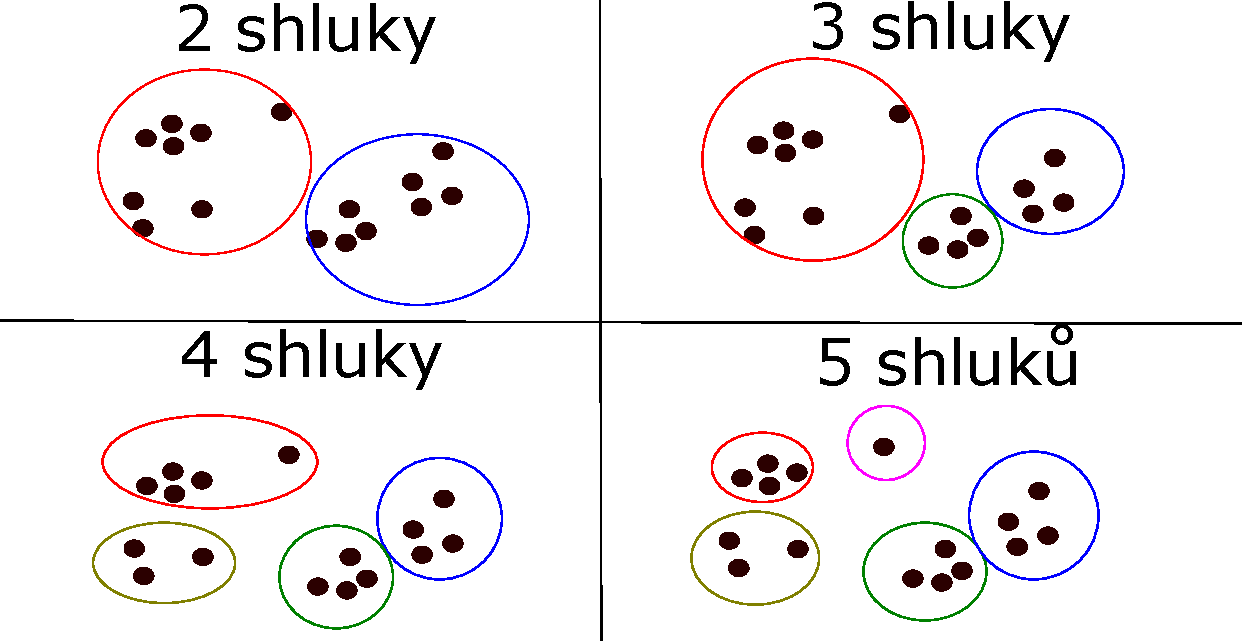
\includegraphics[width=\textwidth]{./img/shlukova_anal}}		
			\caption{Ukázka shlukové analýzy s různým počtem shluků.}
			\label{fig:clustering}
		\end{figure}
		
		\subsection{K-means}
			K-means a K-medoids jsou metody shlukové analýzy. Tyto metody jsou založené na principu centroidů. Centroidem je vyjádřen pomyslný střed každého shluku. V případě K-means jde o střed shluku nezávisle na tom, je-li tento bod i objektem vstupních dat, nebo ne. K-medoids jako střed shluku určí vždy nejvhodnějšího zástupce ze vstupních dat. Graficky je tento rozdíl zobrazen na obrázku \ref{fig:kMeansVSkMedoids}. Z obrázku vyplývá, že shluk v K-means může mít střed mimo data, kdežto K-medoids má možnost středem shluku určit pouze nejvhodnější objekt ze vstupních dat.
			
			Tyto algoritmu patří do kategorie bez učitele. Algoritmy mají na vstupu jednu množinu dat. Na této množině se naučí data třídit do jednotlivých shluků dle podobnosti.
			
			\begin{figure}[htb]\centering
				\tmpframe{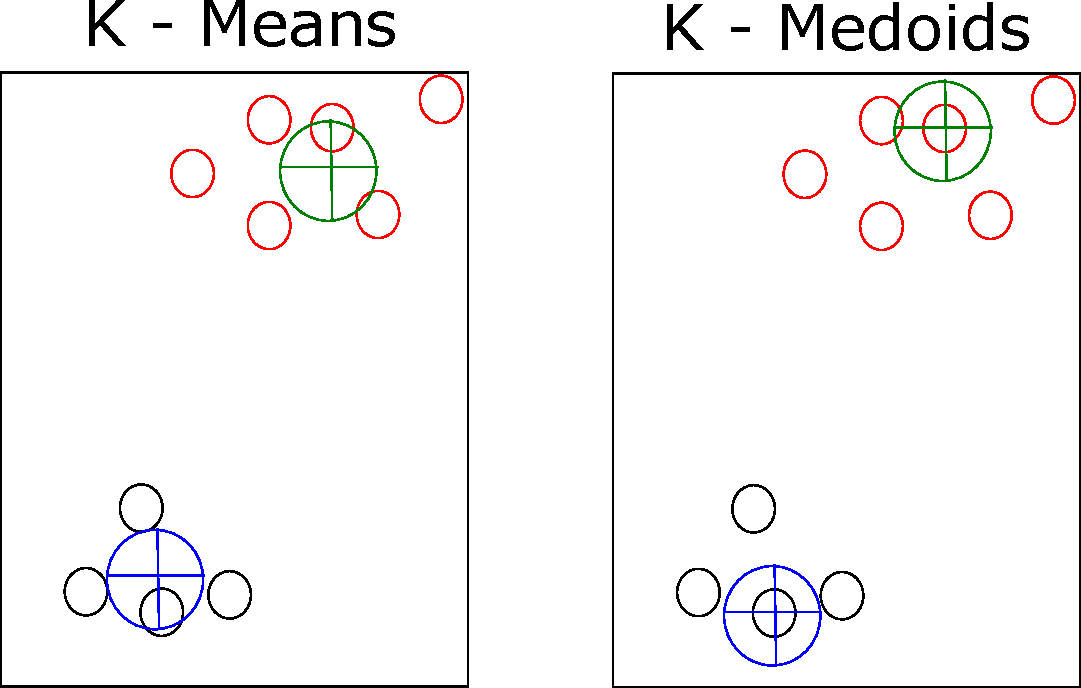
\includegraphics[width=\textwidth]{./img/kmeansVSkmedoids}}		
				\caption{Ukázka shluku a jeho centroidu pomocí metody K-means a K-medoids.}
				\label{fig:kMeansVSkMedoids}
			\end{figure}
		
			Postup algoritmu pro K-means je nejdříve vybrat $K$ bodů jako centroidy. Tyto centroidy lze vybrat například náhodně, nebo prvních $N$. Volbou prvních centroidů se například zabývá zdroj \cite{kMeansInit}. Po vybrání středů se všechny data přiřadí k nejvhodnějšímu shluku. Výběr takové shluku často ovlivňuje například vzdálenost bodu k centroidu. Následuje přepočet nových středů. Přiřazení do shluků a výpočet nových centroidů se opakuje, dokud shluky mění. Po té považujeme algoritmus za hotový a data rozdělená do skupin.
			
			\todo{čeština}
			\begin{minipage}{\linewidth}
				\begin{lstlisting}[caption={Algoritmus K-Means}, label={lst:k-means}]
(1) Nahodn\v{e} vyber k stredu.
(2) Vypocti vzdalenost kazdeho bodu ke vsem stredum.
(3) Prirad bod ke shluku, k jehoz stredu ma nejmensi vzdalenost.
(4) Vypocti nove stredy shluku.
(5) Vypocti nove vzdalenosti bodu ke vsem stredum.
(6) Pokud se zadna data nezmenila skonci. Jinak pokracuj bodem 3.
				\end{lstlisting}
			\end{minipage}
			
			Jedním z kroků algoritmu je přiřadit vstupním objektům správný shluk. K tomuto důvodu je nutné definovat funkci pro měření vzdáleností mezi jednotlivými objekty \cite{IntroductionToDataMining}. Požadavky na takovou funkci jsou, aby byla jednoduchá, protože je velmi často volaná. Pokud data jsou v eukleidovském prostoru používají se například následující funkce na měření vzdálenosti:
			
				\subsubsection{Eukleidova vzdálenost}
				\label{sec:eukleid_distance}
				Eukleidova vzdálenost určuje vzdálenost mezi dvěma body v eukleidově prostoru. Výpočet euiklediovy vzdálenosti mezi body $p = (p_1, p_2, \ldots, p_n)$ a $q = (q_1, q_2, \ldots, q_n)$ je
				$$d_e(p,q) = \sqrt{\sum_{i = 1}^{n}(q_i - p_i)^2}$$
				
				\subsection{Cosinova vzdálenost}
				\label{sec:cosine_distance}
				Cosinova vzdálenost se vypočítá následovně \cite{cosine-similarity}: Máme vektor $A = [A_1,A_2,\ldots,A_n]$ a vektor $B = [B_1,B_2,\ldots,B_n]$. Cosinovu vzdálenost vypočteme jako
				
				$$cos(A,B) = \frac{A*B}{||A|| * ||B||}$$,
				
				kde $||A||$ vyjadřuje velikost vektoru $A$. Stejně tak velikost vektoru $B$ je označena $||B||$.
				
		
				
				\subsubsection{Manhattanská vzdálenost}
				Dalším příkladem měření vzdáleností bodů $p = (p_1, p_2, \ldots, p_n)$ a $q = (q_1, q_2, \ldots, q_n)$ v eukleidově prostoru je manhattanská vzdálenost. Její výpočet je dle vzorce:
				$$d_m(p,q) = \sum_{i = 1}^{n} |p_i - q_i| $$
				
		\subsection{Důvod využití}
			Informace, které integrační platformou prochází jsou velmi různorodé. Požadavky je možné rozdělovat do různých skupin jako například:
			
			\begin{itemize} 
				\item skupiny dle druhu služby (SOAP, REST, databázová \ldots),
				\item skupiny dle služeb (služby na notifikace, na objednávky \ldots),
				\item skupiny dle toho, zdali je zpráva požadavek nebo odpověď.		
			\end{itemize}
		
			Jako jedno z možných rozdělení je možné na požadavky v pořádku, podezřelé požadavky a chybné požadavky. Cílem je najít takovou konfiguraci, která by podobné rozdělení dokázala najít. Tedy rozeznat požadavky, které jsou v pořádku (běžná komunikace na integrační platformě.) od těch, jenž jsou podezřelé (ne příliš častý vzor požadavku, \ldots), či zaručeně chybné (chyba protokolu, validace, \ldots). 
			
			Vhodné rozdělení může být i pouze na podezřelé zprávy a zprávy korektní.		
	
	\section{Detekce anomálie}
		Většina požadavků, která projde skrz integrační platformu jsou v pořádku. Chyba či podezřelá zpráva se vyskytují zpravidla minimálně. Proto jsem jako další metodu zvolil detekci anomálie. Detekce anomálie je proces, při kterém se vyhledávají taková data, která se od ostatních výrazněji liší. Detekování odlišností se hojně využívá právě zajišťování bezpečnosti \cite{AnomDetectPCA}. Příklad anomálie je na obrázku \ref{fig:anomalyInData}, kde jsou červeně zvýrazněné anomálie.
		
		\begin{figure}[htb]\centering
			\tmpframe{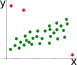
\includegraphics[scale=0.8]{./img/outlier}}		
			\caption{Ukázka anomálií v datech}
			\label{fig:anomalyInData}
		\end{figure}
	
		Princip detekce anomálií je definovat běžná data / chování. Následně veškerá data / chování, která těmto požadavků neodpovídají označit za anomálie \ref{fig:anomalyInData}. 
		
		\subsection{Metody detekce anomálie}
			Detekce anomálií lze rozdělit na tři základní druhy \cite{KumarPCAANom}: 
			\begin{itemize} 
				\item statistické rozdělení
				\item metody založené na vzdálenosti 
				\item metody založené na hustotě		
			\end{itemize}
		
			Statistické metody očekávají, že data mají průběh nějakého statistického rozdělení. Tomu ja následně přizpůsoben přístup zjišťování anomálií. Zpravidla proto tyto metody nejsou v praxi využívané \cite{KumarPCAANom}.
			
			U metod založených na vzdálenosti se vypočítá vzdálenost konkrétního data a jeho sousedů. Je-li nalezena vzdálenost větší než předem daný práh, je cílový prvek chápán jako anomálie.
			
			Metody založené na hustotě vypočítávají takzvaný LOF (Local Outlier Factor). LOF je hodnota, která u každého prvku určuje míru, jako moc je anomálií \cite{LOF}.
			
			Základ výpočtu LOF je, výpočet vzdálenosti ke $k$ nejbližším sousedům. Tato vzdálenost je použita pro odhad hustoty. Následné porovnání hustoty elementu s hustotami svých $k$ sousedů rozhoduje o tom, bude-li označen za anomálii.
			
			Definice LOF dle \cite{LOF} je popsána pomocí několika dílčích definicích: 
			
			\subsubsection{K-vzdálenost}
				Nechť pro libovolné celé číslo $k$, kde $k > 0$ je určena \textit{k-vzdálenost} objektu $p$ ( $k-dist(p)$ ) jako vzdálenost $d(p, o)$, mezi objektem $p$ a objektem $o \in D$, kde platí:
			
				\begin{itemize} 
					\item pro nejméně $k$ objektů $o' \in D \backslash {p}$	platí, že $d(p, o') \leq d(p, o)$ a zároveň
					\item pro alespoň $k-1$ objektů $o' \in D \backslash {p}$ platí, že $d(p, o') < d(p, o)$.
				\end{itemize}
				Množinu $k$ nejbližších sousedů definujeme jako $N_k(p)$
		
			\subsubsection{Dosažitelná vzdálenost}
				Nechť $k$ je přirozené číslo. Dosažitelná vzdálenost objektu $p$ s ohledem na objekt $o$ je definována následovně: 
				$$ reach-dist_k(p, o) = max (k-distance(o), d(p, o)) $$
				
			\subsubsection{Hustota dosažitelnosti}
				Hustota dosažitelnosti objektu $p$ je definována jako
				$$ lrd_{N_k}(p) = \frac{1}{ \frac{\sum_{o \in N_k(p)} reach-dist_k(p,o}{|N_k(p)|}} $$
				
				Hustota dosažitelnosti lze popsat jako inverze průměru dosažitelné vzdálenosti $k$ nejbližších sousedů $p$.
				
			\subsubsection{Činitel anomálie objektu p (LOF)}
				LOF objektu $p$ je definován jako 
				
				$$LOF_{N_k}(p) = \frac{\sum_{o \in N_k(p)} \frac{lrd_{N_k}(o)}{lrd_{N_k}(p)}}{|N_k(p)|} $$
			
			
		
		
		\subsection{Analýza hlavních komponent}
		\label{sec:pca}
		Analýza hlavních komponent, častěji označována jako PCA z anglického překladu \textit{Principal Component Analysis}. \todo{Zkratka PCA} PCA provede analýzu vstupních dat. Tyto data se skládají z mnoha proměnných, které na sobě mohou být závislé. Účelem je vybrat z těchto proměnných důležitou informaci tu reprezentovat jako nové proměnné zvané hlavní komponenty \cite{PCA_book}. Tyto hlavní komponenty jsou lineární kombinací originálních hodnot.
		
	

\chapter{Návrh řešení}
	V této kapitole se zabývám principy, technologiemi a algoritmy, které jsem se rozhodl použít k tomu abych, splnil cíle této práce. Tedy vytvoření aplikace, jenž umožní sledovat bezpečností rizika v reálném čase.
	
	Návrh řešení plyne z toho, že hlavním stavebním kamenem je integrační platforma Unify. Tato platforma využívá již některé metody a standarty. 
	
	\section{Architektura aplikace}
	\todo{Lze rozdělit na podsekce}
	Požadavkem na aplikaci je, aby zprávy zpracovávala a predikovala v reálném časem. Proto je princip položen na čtení požadavků proudících přes platformu. Jejich předzpracování a odeslání do cloudového řešení Microsoft Azure (Více v sekci \ref{sec:ms_azure}). Po přijetí odpovědi je výsledek uložen do databáze. Pro vizualizaci dat slouží REST API \cite{rest}, které vypisuje předem definované informace v ideálním formátu pro zobrazení v Google Charts \cite{googleCharts}.
	
	Pro snazší představu o architektuře aplikace poslouží obrázek \ref{fig:hld_architecture}, na kterém je vidět High Level Desing \cite{hld_johnson}.
	
	\begin{figure}[htb]\centering
		\tmpframe{\includegraphics[width=\textwidth]{./img/jake_HLD}}		
		\caption{High Level Desing aplikace s pracovním názvem JakeTheLogger}
		\label{fig:hld_architecture}
	\end{figure}

	Základem celé aplikace je neohrozit stávající integrační platformu. Proto jsem se rozhodl, že informace o proběhlé komunikaci získám pomocí čtení logovacích souborů.
	Čtením přírůstků k jednotlivým auditovým logům získám chtěné požadavky a pro Unify to nepředstavuje žádnou zátěž.
	
	Dalším stavebním kamenem je použitý aplikační server Jboss ( více v kapitole \ref{sec:jboss}). Na serveru je celá aplikace. Dochází zde k předzpracování zpráv, jejich odeslání do Microsoft Azure (\ref{sec:ms_azure}) a také k ukládání do DB.
	
	Jak jsem již zmiňoval provoz z platformy je po zpracování odesílán do MS Azure, zde jsou definovány jednotlivé algoritmy, jejichž výsledky jsou vracený zpět do aplikačního serveru. Azure jsem se rozhodl používat, protože umožňuje rozložení výkonu na server Microsoftu a protože využití služeb v cloudu se stává stále oblíbenějším. Díky spolupráci s Microsoftem je možné i získat, popřípadě zakoupit, instanci Azure do vlastní sítě. Po diskuzi s Yuriy Zaytsev z týmu Microsoftu jsem získal i potvrzení, že podobné řešení postavené na jboss se v MS Azure nevyskytuje (k březnu 2017).
	
	Získané výsledky jsou zpracovány a uloženy do NoSQL databáze MongoDB (více v kapitole \ref{sec:data_storing}).
	
	Aby výsledky nebyly jen hodnoty uložené v databází, je použité REST API, přes které lze výsledky sdílet. API je navržené tak, aby v případě použití Google Charts nevznikly žádné potíže. 
	
	Google Charts se u cílového zákazníka používají již nyní například na zobrazení stavu objednávek. Proto se jejich použití jeví jako další logický krok. Nicméně, není problém stejné API použít pro svoji libovolnou aplikaci, která hodnoty použije buď pro zobrazování přehledů, nebo jako jeden z dalších vstupů například do různých systémů SIEM.

	\section{Microsoft Azure}
		\label{sec:ms_azure}
		Na integrační platformě Unify \cite{unify} je předpokládaný maximální provoz 20 požadavků za vteřinu. Vzhledem k takto silnému provozu bude potřeba i přiměřeně velký výpočetní výkon. 
			
		Spolupráce se společností Miscrosof \cite{microsoft} mi umožnila jako řešení vyzkoušet její cloudové služby Microsfot Azure \cite{msAzure}.
			
		Microsoft Azure je sada integrovaných cloudových služeb. Azure nabízí cloudová řešení pro mnoho činností. Motivací k použití této služby k detekci bezpečnostních rizik je nástroj Microsoft Azure Machine Learning Studio \cite{msAzureStudio}.
			
		Microsoft Azure Machine Learning Studio je plně cloudová služba, která umožňuje vytváření prediktivních modelů pro strojové učení \cite{msAzureStudio}. Výhodou studia je to, že veškerý výkon je rozprostřen vevnitř cloudu. Díky grafickému rozhraní je snadné vytvořit učící model, který je následně převeden do modelu prediktivního.
			
		Aby měl prediktivní model smysl, je třeba mu poskytovat nějaká data, u kterých je predikce využita. K tomu se využívají webové služby.
		Prediktivní model se vystaví na specifické URL adrese. Zde je pak očekáván na vstupu konkrétní formát JSONu a služba vrací předem definovanou odpoveď se správnými parametry.
		
		Výhodou využití cloudu je přenesení výpočetní zatěže mimo společnost. Naopak rizikem je problém s konektivitou, který může vytvořit výpadek služby a nebude tedy možné po tuto dobu predikovat rizika. Jednou z možností, jak řešit takové riziko je nechat přenést instanci MS Azure do své sítě.
		
		\subsection{Prostředí Microsoft Azure Machine Learning Studio}
			Azure Machine Learning Studio (dále jako Azure nebo MS Azure) usnadňuje vytváření algoritmu pro strojové učení. Úvodní obrazovka grafického rozhraní je zobrazena na obrázku \ref{fig:MSAzureML}.
			
			\begin{figure}[htb]\centering
				\tmpframe{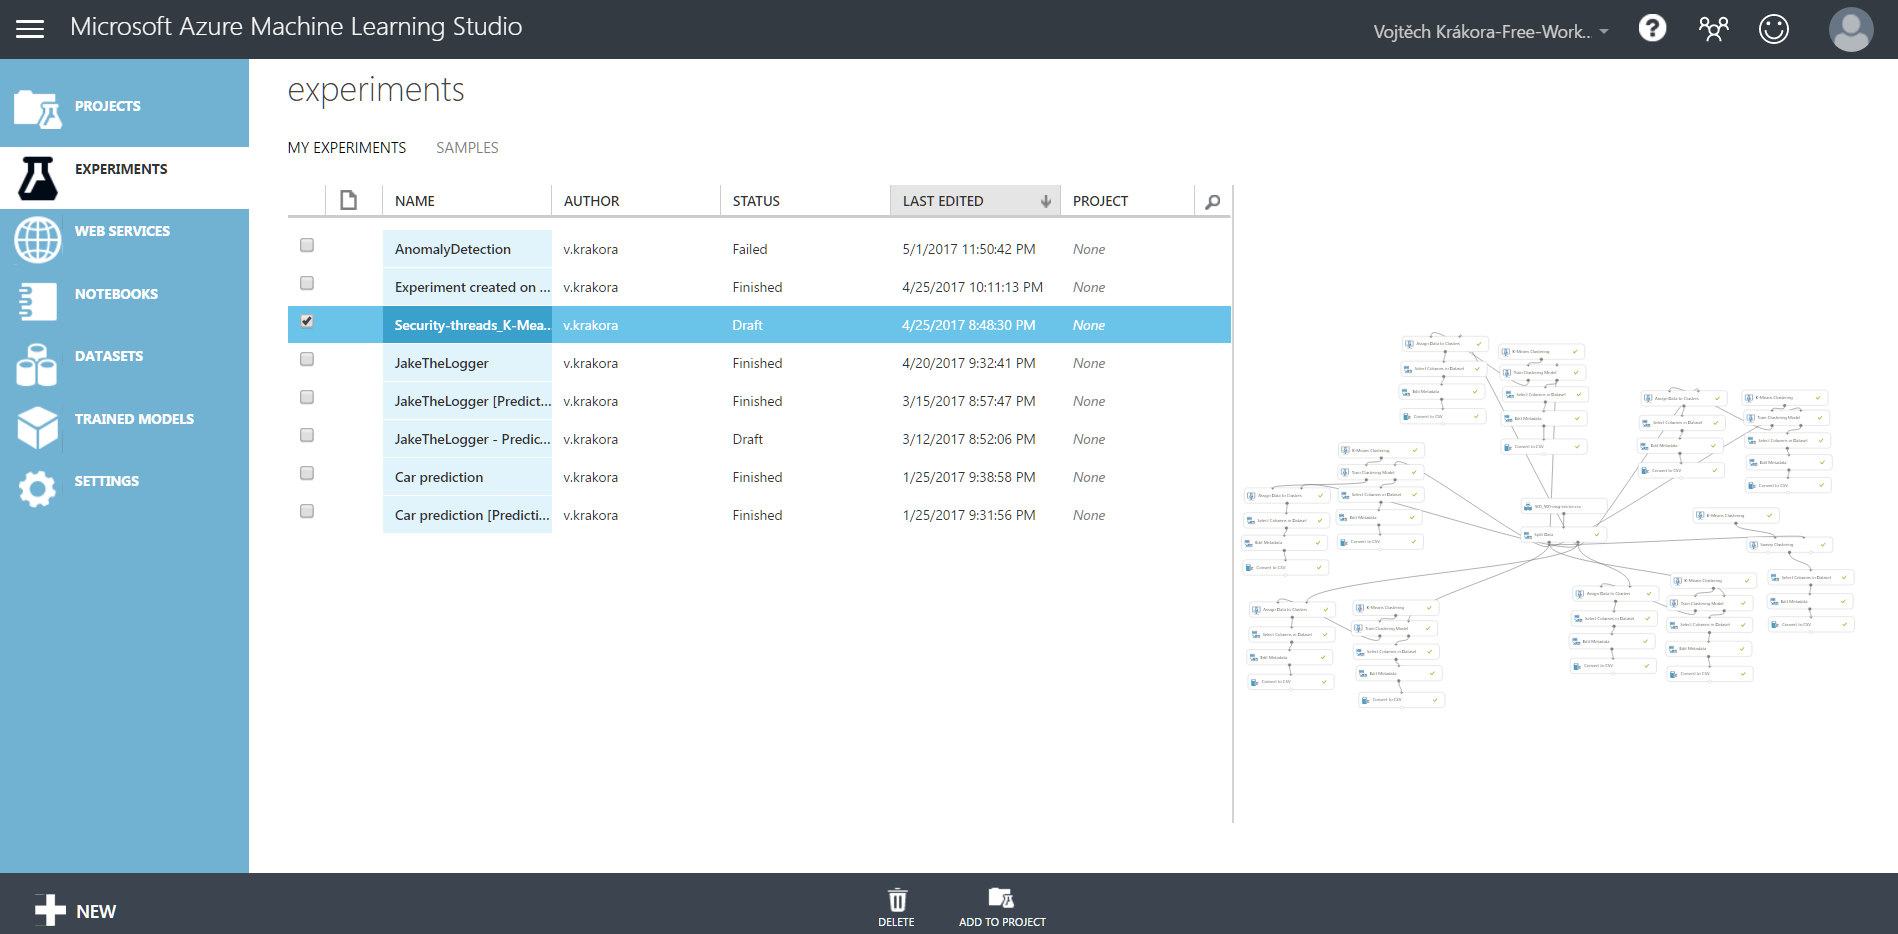
\includegraphics[width=\textwidth]{./img/MSAzureML}}		
				\caption{Grafické rozhraní Microsoft Azure Machine Learning Studia}
				\label{fig:MSAzureML}
			\end{figure}
			
			Základem veškerých experimentů jsou vstupní data. Ty lze do Azure uložit jako vlastní dataset. Data mohou být předzpracována, ale není to podmínkou. Azure poskytuje řadu nástrojů pro přípravu dat a stejně tak i možnost vytvoření vlastních komponent napsaných v jazyce R nebo Python.
			
			Samotný experiment se skládá z jednotlivých komponent. Ty jsou tedy buď již definované nebo vlastní. Experimenty jsou děleny na trénovací experimenty a na prediktivní. Trénovací experiment je takový, který naučí celý experiment predikovat data. Nachází se v něm zpravidla trénovací množina (může být rozdělena dále i na validační část), vybrané komponenty představující algoritmy strojového učení a prvky zobrazující výsledky. Mezi těmito hlavními částmi se mohou vyskytovat další komponenty například pro předzpracování dat, rozdělení dat, validaci, stažení a podobně. Pokud jsme s výsledky trénovacího experimentu spokojení může být automaticky vygenerován experiment prediktivní. Ten je připraven na vstup získat data a vrátit výsledky z naučeného algoritmu. Takový experiment je možné vystavit jako webovou službu.
			
			Další záložky obsahují poznámky nebo například vystavené webové služby.
			
			
		
	\section{JBoss}
		\label{sec:jboss}
		Základem integrační platformy Unify je aplikační server JBoss AS 7 \cite{unify}. Je potřeba, aby cílový aplikace byla kompatibilní, proto se i její vývoj bude soustředit na nasazení na JBoss.
		
		Jboss AS je aplikační server pro Javu EE\cite{jboss}.

					
	\section{Logování Unify}
		\label{sec:logging_unify}
		Abychom nenarušil novou komponentou provoz platformy, budou veškeré zprávy, které přes ni budou vedeny čteny z logu. Platforma Unify loguje veškerý průběh do souborových logů. Protože celá integrace je založena na Javě, je využit logovací framework Log4j \cite{log4j}.
		Každý požadavek, který na platformu přijde je zalogován do audit.logu. Zpráva je vždy na jedné řádce a zároveň na jedné řádce je povolena pouze jedna zpráva.
		
		\begin{minipage}{\linewidth}
			\begin{lstlisting}[caption={Část řádky v auditovém logu Unify}, label={lst:log}]
REQ;20170117;16:03:01;WorkRequestMgmtService;
cancelOrderedService;esb1-1484665381312-5369
			\end{lstlisting}
		\end{minipage}
		
		Jedna řádka auditového logu obsahuje:
		
		\begin{itemize} 
			\item informaci o čase zápisu,
			\item závažnost z pohledu javy, 
			\item název třídy, který uložil řádku do logu,
			\item název vlákna, který zapisovanou část zpracovával,
			\item informaci zda je o požadavek (REQ) nebo odpověď (RES), či chyby (ERR),
			\item datum přijetí požadavku,
			\item čas přijetí požadavku,
			\item název logující komponenty,
			\item název operace,
			\item jednoznačný identifikátor požadavku,
			\item obsah požadavku.		
		\end{itemize}
		
		Jednotlivé části logu jsou od sebe odděleny středníkem.
		
		Vzhledem k tomuto principu jsem se rozhodl přistoupit k tomu, že se vybrané logovací soubory budou kontinuálně číst, kde se bude ke každému řádku přistupovat jako k samostatné zprávě, která bude následně zpracována dál.
		
		Díky této volbě nebude nutné nijak zasahovat do integrační platformy Unify a minimalizuje se tím riziko, jakéhokoliv nebezpečí ze strany této aplikace.
		
		Unify využívá pro některé služby logování do Oracle databáze. Ale vzhledem k tomu, že jde pouze o několik málo určených služeb, připojení na databázi by tak kromě případných komplikací ani nepřineslo žádaný účinek. Veškerá komunikace ukládaná do databáze je stejně duplikovaná i v logovacích souborech.
					
	\section{Předzpracování dat}
		\label{sec:preprocessing}
		
		Pro snazší práci s informacemi z logů jsem se rozhodl pro normalizaci jednotlivých požadavků. Normalizace je jeden z požadavků při zpracovávání textu \cite{txtNrmlztn}.
		
		V kapitole \ref{sec:logging_unify} jsou vidět informace, které se kromě samotné zprávy logují. V každé zprávě se objevuje takzvaná integrační hlavička. V té jsou základní údaje, jako čas odeslání, jednoznačné identifikátory, zdrojové a cílové systémy. Položka jako je časové razítko bude zpravidla pro každý požadavek jiná, stejně na tom budou jednoznačné identifikátory. Z tohoto důvodu jsem se rozhodl zvolit jejich nahrazení.
		
		Při normalizaci dat jsem se podobně jako ve zdroji \cite{Li_2013} rozhodl použít následovně:
		
		\begin{itemize} 
			\item nahrazení všech čísel - pomocí speciálního symbolu \uv{\#} nahradím všechny výskyty čísel,
			\item velikost písmem - všechna písmena jsou z velkých znaků převedena na znaky malé,
			\item nahrazení speciálních znaků -veškeré znaky jako jsou čárka, tečka \ldots jsou nahrazeny mezerou,
			\item odstranění xml tagů - rozhodl jsem zpracovávat jen obsah zpráv bez XML tagů.	
		\end{itemize}
	
		Nahrazení čísel se mi jeví jako logický krok. V jednotlivých požadavcích jsou čísla výsledky různých měření na sítí nebo právě časové razítko. Pro další využití považuji za podstatné vědět, že se v daném místě vyskytovalo číslo, než že to bylo nějaké konkrétní číslo.
		
		Převod písmen na malá zajistí, aby slova, lišící se právě jen ve velikosti nějakých písmen byla vyhodnocena jako stejná.
		
		Veškerá komunikace na platformě je převedena do XML (není-li již od počátku vedena v XML). Protože téměř u všech zpráv stejného druhu se používají ty samé XML tagy, nebudou pro další zpracování podstatné a budou zcela odstraněny. Algoritmus bude dále pracovat jen s reálným a normalizovaným obsahem zprávy. 
		
	 	Pro ilustraci normalizace poslouží následující ilustrační příklad:
	 	
	 	\begin{minipage}{\linewidth}
	 		\begin{lstlisting}[caption={Ilustrační příklad XML požadavku}, label={lst:xml-example}]
<WebService>
  <header>
    <timestamp>2016-08-09T11:11:11</timestamp>
  </header>
  <body>
    <firstElement>Hello world!</firstElement>
    <secondElement>0</secondElement>
  </body>
</WebService>
	 		\end{lstlisting}
	 	\end{minipage}
			
			ten by normalizaci vypadal následovně:
			
			\begin{minipage}{\linewidth}
				\begin{lstlisting}[caption={Ilustrační příklad po normalizaci}, label={lst:xml-example-normalized}]
# # #T# # # hello world #
				\end{lstlisting}
			\end{minipage}
		
		Čištění dat probíhá na straně aplikace. Do MS Azure tedy chodí už pouze korektní vstupní data. Vyčištění se stará o to, že nekorektní požadavky nejsou zpracovány. Je to pojistka proto, kdyby nějaká zpráva byla více řádková (například nechtěnou změnou logování). V takovém případě se nepodaří pomocí regulárního výrazu najít jednoznačný identifikátor platformy a \uv{požadavek} je ignorován.
			
	\section{Vytvoření vektoru}
		\label{sec:construct_vector}
		
		\subsection{Forma vektoru}
		V sekci \ref{subsec:tf-idf} jsem navrhl, jak textová data převést do vektoru. Tím je zaručené, že bodou-li se data přenášet přes internet do Microsoft Azure, budou anonymizována. Z vektoru nedokážeme zpětně zprávu vyčíst.
		
		I když z Azure dostáváme synchronně odpověď zpět, a je tedy jasné, ke které zpráve dostávám výsledek, rozhodl jsem se odesílat i jednoznačný identifikátor platformy. To vede k tomu, že pro znalého člověka lze jednotlivé požadavky sledovat i uvnitř MS Azure. Identifikátor sám o sobě vypovídající hodnotu žádnou nemá, ale máme-li k dispozici původní zprávu, jsem ji schopni dohledat.
		
		\todo{Ukázka vektoru}
		
	\section{Konstrukce clusteringu}
		\label{sec:construc_clustering}
		Microsoft Azure nabízí k přípravě experimentů svoje studio dostupné na adrese \url{https://studio.azureml.net}.
		
		Ve studiu Azureml je možné vytvářet své projekty, do projektů umístit své experimenty a ty následně vystavit jako webovou službu.
		
		Základem úspěšného experimentu je vytvořit učící model. To je takový model, pro který máme zvolený cílový algoritmus a na předpřipravených datech ho naučíme aby dokázal v našem případě co nejlépe rozdělovat zprávy do clusterů.
		
		\subsubsection{Předzpracování}
		Veškeré předzpracování a čištění dat probíhá v mojí aplikaci i přesto jsem základní předzpracování zvolil i do experimentu samotného.
		
		Po načtení vstupních dat dochází odstranění duplicitních řádků. Jako další metoda je využití modulu, který smaže řádky, jimž chybí nějaká data.
		
		\todo{Mohl bych použít zároven s klasifikacnim modelem, ale nevim.}
		\subsubsection{Zpracování}
		Pro zpracování jsem zvolil K-Means modul, který je připojený na modul pro trénování clusterovacích modulů.
		
		Po natrénování přiřadíme zbytku testovacích dat clustery a může zhlédnout výsledek.
		
		Na obrázku \ref{fig:k-means_azure} je vidět celý vytvořený trénovací experiment.
		
		
		\begin{figure}[htb]\centering
			\tmpframe{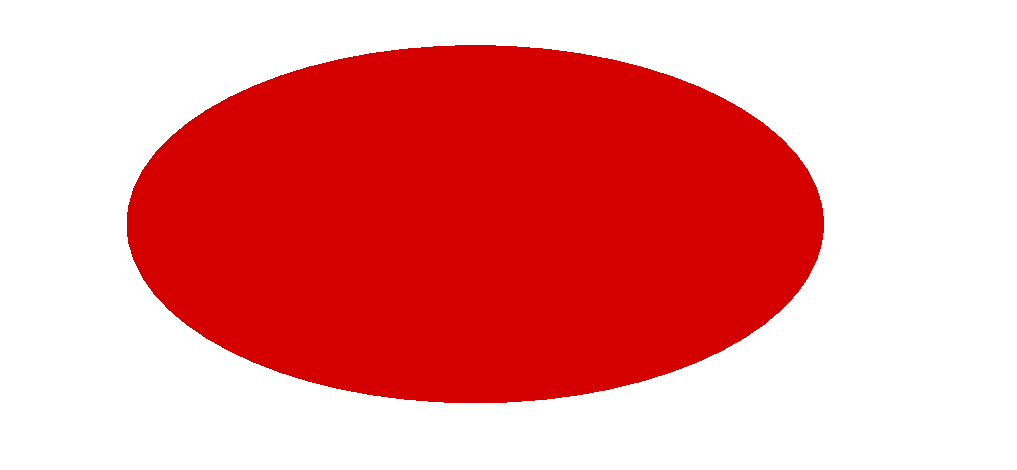
\includegraphics[width=\textwidth]{./img/todo}}	
			\caption{Clustering k-means v prostředí MS AZURE ML Studio.}
			\label{fig:k-means_azure}
		\end{figure}
		
		\todo{Doplnit sem ukázku přiřazení dat a grafy z azure}
		\todo {jak jsem zjistil nejlepší vhodné nastavení}
		
	\section{Konstrukce detekce anomálie}
		\label{sec:construc_anomaly}
		Druhou možností, kterou bych rád vyzkoušel je detekce anomálie.
		To, že chybné požadavky nebo bezpečnostní požadavky se budou výrazněji lišit od běžných zpráv se dá předpokládat.
		
		Princip předzpracování dat v Azureml studiu je stejný jako v při konstrukci modelu pro clustering. Řádky s chybějícími hodnotami a duplikované pro trénování nebudeme používat.
		
		Kromě výše uvedené předzpracující části i zde je část učící a část vyhodnovací.
		
		Trénovací model je vidět na obrázku \ref{fig:anomaly_detection_azure}.
		
		\begin{figure}[htb]\centering
			\tmpframe{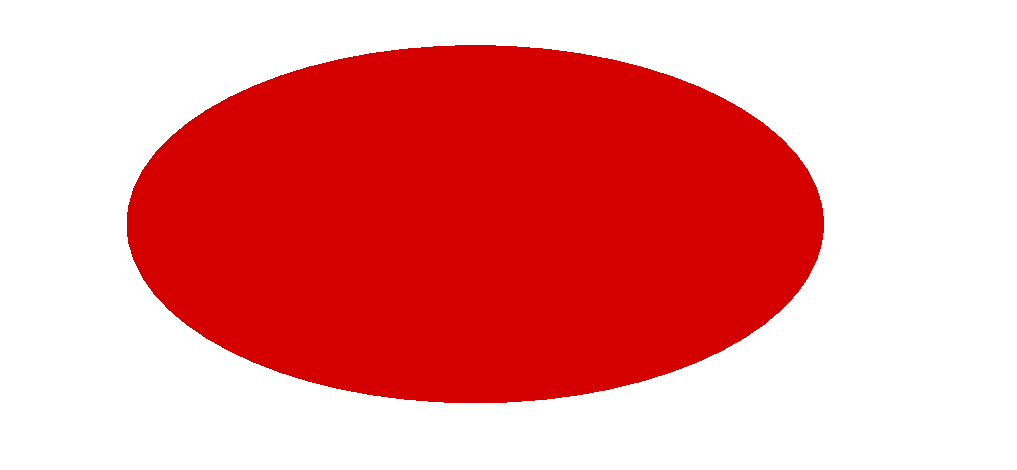
\includegraphics[width=\textwidth]{./img/todo}}	
			\caption{Detekce anomálií v prostředí MS AZURE ML Studio.}
			\label{fig:anomaly_detection_azure}
		\end{figure}
		\todo {jak jsem zjistil nejlepší vhodné nastavení}
		
	\section{Ukládání dat}
	\label{sec:data_storing}
	Rozhodl jsem se pro ukládání dat využít NoSQL databázi. Protože aplikace Unify momentálně ukládá veškerý svůj provoz do souborů (výjimečně jsou některé konkrétní služby journalovány do DB), bude databáze využita i pro ukládání veškeré komunikace. To zpřístupní do budoucna snazší operování s jednotlivými zprávami. Popřípadě jednoduší zpětnou analýzu.
	\todo{Schéma DB}
	
	
	Protože se bude ukládat veškerá komunikace, rozhodl jsem se v databázi mít uvedené následující informace:
	
	
	\begin{itemize} 
		\item ObjectId - automaticky generováno z MongoDB,
		\item timestamp- časové razítko uložení záznamu do DB,
		\item original-message - nezměněná zpráva,
		\item normalized-message - zpráva po normalizaci,
		\item platformId - jedinečný identifikátor platformy,
		\item assignment - skupina, kterou azure vyhodnotil pro zprávu jako správnou. 		
	\end{itemize}
		
	\section{Prezentace dat}
		\label{sec:data_prezentation}
		Vzhledem k tomu, že by aplikace měla být schopna určovat bezpečnostní rizika, je třeba nějakým způsobem prezentovat její výstupy. Moninitoring na aplikaci Unify je momentálně postaven na tom, že konkrétní lidé hlídají logy a v případě vyskytu chyb, varování nebo jiné netypické události zjišťují co bylo příčinou.
		
		Rozhodl jsem se tedy, že nejlepší bude grafické znázornění. Kromě údajů o tom, že byl zaznamenán požadavek, který je podezřelý budu grafy využívat i k prezentaci základního monitoringu. 
		
		Vzhledem k tomu, že se bude veškerá komunikace ukladát bude vhodné prezentovat například i kolik požadavků na jednotlivé komponentě proběhlo za poslední hodinu a podobně.
		
		Společnost Cetin a.s. \cite{cetin} ve které bude aplikace testována a jenž je uživatelem integrační platformy používá pro různá grafická znázornění grafy od Google Charts\cite{googleCharts}. 
		
		Tyto grafy jsou napsané v jazyce Javascript. Je tedy možné jejich umístění například na intranetové stránky, kde se vysoce postavení lidé společnosti vyznají lépe než v jednotlivých monitorovacích aplikacích.
		
		Na tomto základě jsem se rozhodl vytvořit REST API \cite{rest}, jenž budou Google Charts schopny snadno konzumovat a v případné jiné aplikace, které by stály o podobná data budou schopny se jim přizpůsobit.
		
	\section{Využití dát systémy 3. stran}
		Do budoucna je potřeba počítat s rozšířením monitoringu a je proto vhodné aplikaci připravit tak, aby její výsledky mohly být využity v aplikacích 3. stran.
		
		Lze předpokládat, že k monirování bezpečnosti provozu budou použity systémy SIEM (Security Information and Event Management) \cite{siem}.
		SIEM funguje na principu, kdy zpracovává co nejvíce údajú, na jejichž základě pak rozeznává neočekávané situace a rizika \cite{howDesSiemWork}.
		
		Tím, že jsem se rozhodl data ukládat tak, jak uvádím v kapitole \ref{sec:data_storing} bude libovolný SIEM po připojení do DB schopen získat jak originální zprávu, tak její normalizovanou verzi popřípadě i výsledek vyhodnocení mé aplikace.
		
		Dále je možnost napojit SIEM i na REST API obdobně jako Google Charts v kapitole \ref{sec:data_prezentation}.
		
\chapter{Realizace}
	\todo{Sem vepsat nějaký úvod k této kapitole}
	
	\section{Nutné přípravy pro jboss}
		\subsection{Připravení modulů}
		V aplikaci využívám různé java knihovny, abych k nim měl přístup i v aplikačním serveru, je nutné do něj přidat speciální modul.
		
		Jboss umožňuje snadné přidání modulů. Veškeré moduly jsou umístěny v \textit{wildfly/jboss-eap-7.0/modules/system/layers}. Zde jsem vytvořil svůj modul s konkrétními java knihovnami:
		\begin{itemize} 
			\item commons-codec-1.10.jar
			\item json-simple-1.1.1.jar
			\item mongo-java-driver-3.4.2.jar		
		\end{itemize}
		
		\subsection{Port offset}
		\todo{Je možné, že offset ve finále ještě změním.}
		Dále bylo nutné pro jboss nastavit portový offset. Protože na serveru není jedinou aplikací, je běžný problém v kolizi portů. Z tohoto důvodu jsem zvolil offset 10000. Webové služby tedy místo portu 8080 běží na portu 18080.
		
		\subsection{Zapnutí CORS}
		CORS (Cross-origin resource sharing) neboli \textit{sdílené zdroje odjinud} umožňuje odesílání odpovědí na požadavky z jiné domény \cite{CORS}. V aplikaci je to potřebné pro rest api, kterého se následně dotazuje Google charts.
		
		Corse se v Jboss povoluje v konfiguračním souboru pro standalone aplikaci \textit{standalone.xml} pro doménovou \textit{domain.xml}.
		
	
	\section{Vytvoření modelu na Azure}
		\todo{Ukázka URL}
		\todo{Ukázka Vstupního JSONu a výstupního}
		\todo{V této části bude Prediktivní algoritmus}
		\subsection{Clustering v Azure}
			\todo{Popsat prediktivní experiment}
			\blind[1]
		\begin{figure}[htb]\centering
			\tmpframe{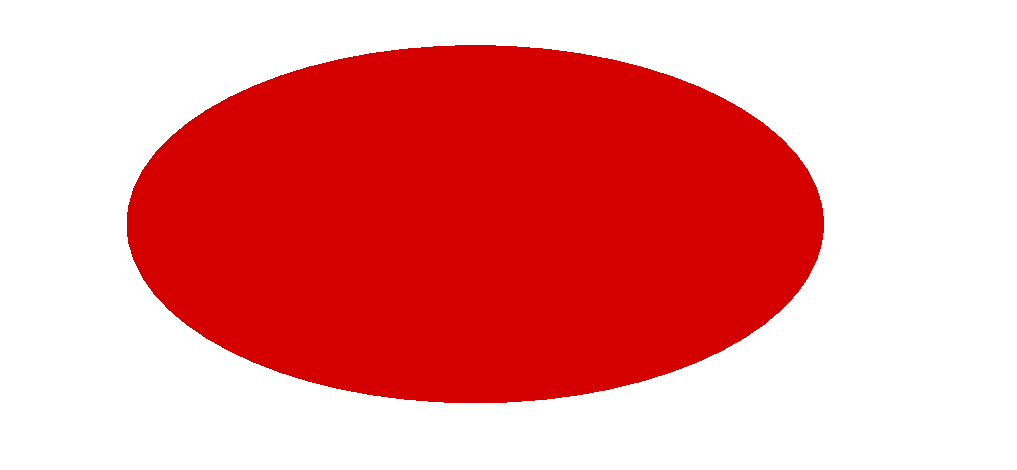
\includegraphics[width=\textwidth]{./img/todo}}	
			\caption{Prediktivní model clusteringu v Azure.}
			\label{fig:training_clustering_azure}
		\end{figure}
		
		\subsection{Detekce anomálií v Azure}
			\todo{Popsat prediktivní experiment}
			\blind[1]
		\begin{figure}[htb]\centering
			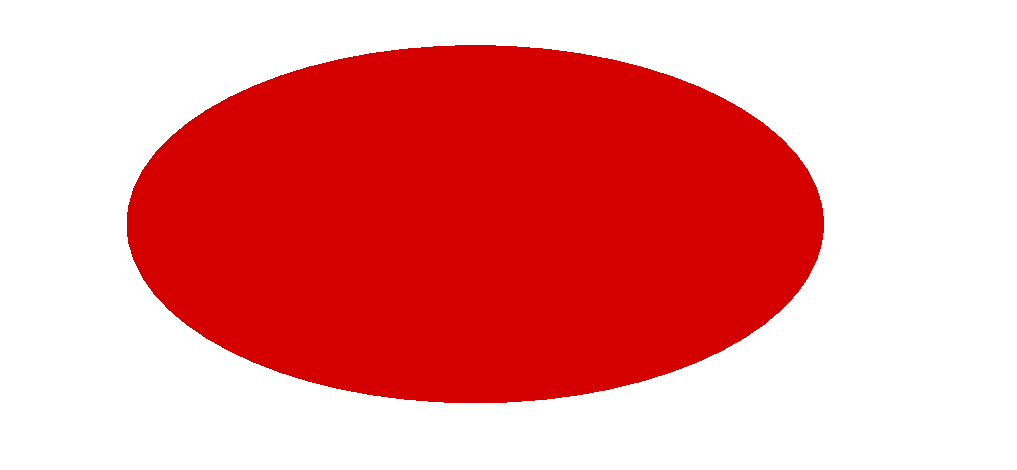
\includegraphics[width=\textwidth]{./img/todo}
			\caption{Prediktivní model v detekci anomálií v Azure.}
			\label{fig:training_anomaly_azure}
		\end{figure}
	
		\subsection{Webová služba}
			Po dokončení prediktivního modelu je třeba experiment vystavit tak, abychom ho mohli používat z vlastní sítě.
			
			Azure umožňuje takový model spustit jako webovou službu.
			
			  \begin{figure}[htb]\centering
			  	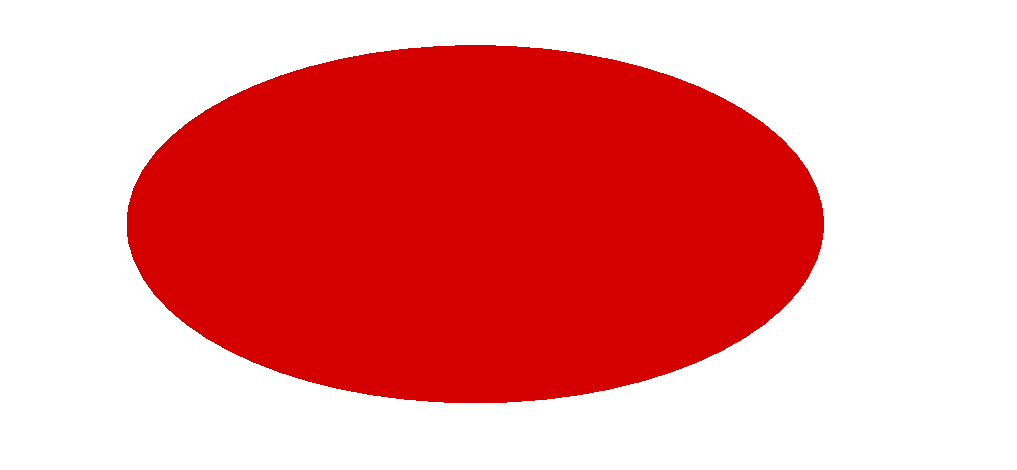
\includegraphics[width=\textwidth]{./img/todo}
			  	\caption{Vytvoření webové služby pomocí stisku tlačítka.}
			  	\label{fig:azure_create_web_servise}
			  \end{figure}
		  
		  Po vytvoření webové služby získáme takzvaný \uv{API key}. Tento řetězec bude sloužit pro přihlášení se do Azure, při dotazování se na konkrétní službu.
		  
		  Také je možné službu otestovat. Otevře se nám okno s očekávanýma políčkama (obr. \ref{fig:azure_test_web_service}). Po vyplnění políček se zobrazí odpověď z prediktivního modelu. Tímto způsobem můžeme otestovat funkčnost nebo pár vzorků. Jiná použití by byla velmi časově a zdrojově nevýhodná.
		  
		  \begin{figure}[htb]\centering
		  	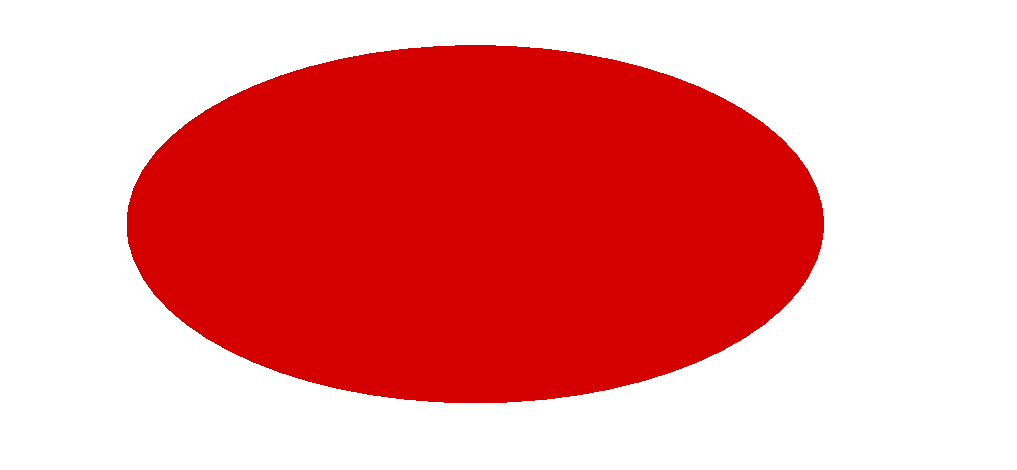
\includegraphics[width=\textwidth]{./img/todo}
		  	\caption{Zobrazené okno pro otestování prediktivního modelu jako webové služby}
		  	\label{fig:azure_test_web_service}
		  \end{figure}
	
	\section{MongoDB}
	\todo{Celkově z této sekce jsem rozpačitý}
		Pro potřeby aplikace je nutné v co nejrychlejším možném čase ukládat jednotlivé requesty. Při ohromném provoze, který se na integrační platformě vyskytuje to je nutná podmínka pro to, aby bylo možné v reálném čase jednotlivé požadavky zpracovávat.
		
		\begin{figure}[htb]\centering
			\tmpframe{
\includegraphics[width=0.2\linewidth]{./img/todoSmall}}	
			\caption{Logo MongoDB. \cite{mongoDB}}
			\label{fig:mongodb_logo}
		\end{figure}
		
		Rozhodl jsem se za tímto účelem využít MongoDB \cite{mongoDB}, protože se očekává, že bude třeba ukládat v mimořádném případě až 30 záznamů za sekundu, zpravidla bude docházet k více zapisům než čtením.
		
		\subsection{NoSQL}
			MongoDB patří do takzvaných NoSQL databází \cite{mongoDB}. NoSQL v angličtině znamená \uv{Not Only SQL} \cite{Moniruzzaman_2013}, v překladu \uv{Nikoliv pouze SQL}. Jde o skupinu nerelačních databází. Takové databáze nejsou primárně postavené na principu tabulek a zpravidla nepoužívají SQL pro práci s daty \cite{Moniruzzaman_2013}.
			
		\subsection{O MongoDB}
			MongoDB je licencovaná pod  GNU AGPL v3.0 \cite{mongo_gnu} licencí. Data jsou ukládána ve formátu BSON. BSON je binárně zakódovaná JSON \cite{bsonspec.org}.
			
			V MongoDB se vytvářejí kolekce, každá kolekce obsahuje soubory. Soubory mají parametry \cite{mongoDB}. Soubory a jejich parametry lze v čase libovlně měnit nebo přidávat. Což je výhoda, pokud zjistíme, že aktuální návrh není finální, vyhneme se problémům s migrací do nového schématu.
			
			V rámci souboru je možné definovat čítač, který se využije k tomu, aby automaticky generoval jednoznačný identifikátor k souborům nebo lze využít parametr souboru \textbf{\_id}. Ten vygeneruje jednoznačnou identifikaci, ze které jsme schopni například získat i čas vložení dokumentu do kolekce. 
			
		\subsection{Využití v práci}
			\subsubsection{Kolekce terms}
			V práci využívám databázi k ukládání všech slov, ze kterých se tvoří vektor, jenž reprezentuje konkrétní požadavek ( více v kapitole \ref{sec:construct_vector}). Tím není potřeba je mít v paměti a při připadném výpadku je znova vypočítávat.
			
			 V kolekci \textit{terms} ukládám soubory jejichž struktura je automatický identifikátor, slovo pro konstrukci vekotru a timestamp přidání dokumentu do kolekce.
			
			\subsubsection{Kolekce messages}
			Další kolekcí je kolekce \textit{messages}. V té jsou uložené veškeré požadavky, které byly přečteny z logů integrační platformy. Protože ještě před uložením do kolekce dochází v Azure k vyhodnocení, je zpráva uložené i s informací, která určuje zdali je požadavek vyhodnocen jako bezpečností riziko nebo není. 
			
			Struktura každého souboru je: 
			
			\begin{itemize} 
				\item \textbf{\_id} - automaticky generovaný identifikátor
				\item \textbf{timestamp} - čas uložení souboru
				\item \textbf{original-message} - původní požadavek, tak jak byl převzat z logu integrační platformy
				\item \textbf{normalized-message} - požadavek ve znormalizované podobě
				\item \textbf{platform-id} - jednoznačný identifikátor v rámci integrační platformy
				\item \textbf{assignment} - informace od Azure s výsledkem přiřazení katogire 	
			\end{itemize}
		
		\todo{Lépe vysvětlit assignment}
		\todo{Konfigurační kolekce}
		
		\subsection{Práce s MongoDB v Javě}
		V implementaci jsem vytvořil třídu \textit{MongoClientService} (aby bylo možné třídy využívat i v jiných modulech, musí se taková třída skládat z interfacu a jeho implementace, v textu se budu bavit o celku implementace a interfacu dohromady například jako o třídě MongoClientService). Tato třída umožňuje distribuci konkrétní databáZe napříč celou aplikací. 
		
		V jednotlivých modulech si vyvoláme instanci konkrétní databáze a nad tou jsme schopni pracovat. Ovladače pro MongoDB nám umožňují jak data v kládat, tak je číst.
		
		
		
		
	\section{Čtení dat z logů}
		\todo{Popis}				
		Při návrhu zisku jednotlivých požadavků z integrační platformy jsem vycházel z toho, že nový aplikace musí minimálně, či spíše vůbec nezatěžovat Unify \cite{unify}. Vzhledem k tomu, že přes integraci proudí veškerý provoz, je sama o sobě dosti vytížená a v případě, že by touto aplikací byl způsoben výpadek došlo by k silnému ztížení veškerých bussiness procesů, což si nelze dovolit.
		
		Unify veškeré požadavky ukládá do logovacích souborů. Některé, převážně rizikové, služby se zároveň ukládají Oracle databáze. Ale vzhledem k tomu, že nejde o všechny dostupné služby rozhodl jsem se toho nevyužít.
		
		Princip získání dat proudicích přes integrační platformu je založen na čtení jednotlivých logovacích souborů. Jako vhodný nástroj jsem vybral Java třídu Tailer z dostupné knihovny org.apache.commons.io \cite{tailerClass}.
		
		Třída \textit{Tailer}, po implementaci listeneru, se chová stejně jako linuxový příkaz tail \cite{tailLinux}. Průběžně kontroluje čtený soubor a každou nově zapsanou řádku zpracovává.
		
		Tímto řešením získáváme data z integrační platformy, aniž bychom jí zatěžovali. 
		
	\section{Předzpracování a odeslání do Azure}
		\label{sec:send_to_azure}
		\todo{Možná rozdělit na dvě sekce}
		
		Protože jsou data odesílána do cloudu, předzpracováváme je lokálně a přímo do Microsfot Azure odesíláme už jen identifikátor zprávy a vypočtený vektor.
		
		Po přečtení zprávy z auditového logu Unify je zpráva předzpracována (\ref{sec:preprocessing}) a následně je z ní vytvořen vektor (\ref{sec:construct_vector}).
		
		\subsection{Start aplikace}
			První start aplikace je komplikovanější v tom, že pro výpočet finálního vektoru ještě nemáme známá vhodná slova, pro která se budou TF a IDF vypočítávat.
			
			Pro případ, kdy je databáze zcela prázdná jsou nejdříve načteny nějaké zprávy (dle konfigurace), z těch jsou vypočetent vhodné termy.
			V případě, že databáze nějaké zprávy již obsahuje je možné využít je. Nedoporučovaný způsob je vložení slov přímo do databáze. Tato metoda může být vhodná v případě, že například chceme databázi migrovat a nechceme se zdržovat znovu výpočtem.
		
		\subsection{Získání dat z logu}
		 Samotný zisk dat z logu je řešen pomocí Java knihovny Tailer \cite{javaTailer}. Jednou z věcí, které bylo potřeba vyřešit byla situace, kdy třída Tailer během čekání na nový přírustek logovacího souboru zcela zablokovala program. Situaci jsem vyřešil tím, že procesu, který čte z logu integrační platformy jsem pomocí \textit{ExecutorService} \cite{javaExecutorService} umožnil běžet na pozadí aplikace. Tím jsem neblokoval řízení programu.
		 
		\subsection{Předzpracování dat}
		Celý proces předzpracování zpráv probíhá v implementované třídě \textit{LogListener}. Po získání dat, jako textového řetězce, jsou uložena do struktury třídy \textit{AuditLogMessage} (obr \ref{fig:auditLogMessage}). 
		
		Následuje proces vytvoření vektoru, který je odesílán do MS Azure. Vektor se vytváří dle pravidel uvedených v sekci \ref{sec:construct_vector} včetně všech procesů předzpracování . Metody pro výpočet TF a IDF jsou implementované ve třídě \textit{WeightsCounterService}.  
		
		Vektor samotný je reprezentován jako seznam \textit{Double} čísel.
		
		\begin{figure}[htb]\centering
			\tmpframe{
\includegraphics[width=0.2\linewidth]{./img/todoSmall}}	
			\caption{Struktura třídy AuditLogMessage.}
			\label{fig:auditLogMessage}
		\end{figure}
		
		Pro odeslání dat bylo třeba vytvořit třídu \textit{AzureWebService}. Vytvoření vhodného požadavku na Azure je podmíněno přihlášením se do služby. Proto do hlavičky je přidána \textit{Basic Access authentication} (jednoduché ověření přístup).
		
		Na požadavek ihned dostaneme synchroní odpověď s výsledkem. Výsledek je zpracován a přiložen k datům načteným z logu.
					
		
	\section{Uložení dat}
	
		\subsection{Kolekce}
		Do databáze se dvě kolekce:
		
		\begin{itemize} 
			\item terms	
			\item messages			
		\end{itemize}
	
		Tyto kolekce (znázornění také na obrázku \ref{fig:colections}) jsou využívány při běhu programu. 
		
		Kolekce \textit{terms} slouží k uchování výrazů, které se používají pro výpočet TF-IDF (kapitola \ref{sec:construct_vector}). \todo{Popsat strukturu kolekce}
		
		Kolekce \textit{messages} uchovává veškeré požadavky a to jak v jejich originální podobě (parametr original-message), tak její normalizovanou metodu (normalized-message). Podstatným identifikátorem každého požadavku je jeho unikátní ID v rámci platformy Unify. Pro tento účel je použit parametr platformId. Posledním parametrem této kolekce je assignment. Tento parametr uchovává informaci o tom, do jaké (rizikové) kategorie byl dle algoritmu běžícím v MS Azure zařazen.
				 
		
		\begin{figure}[htb]\centering
			\tmpframe{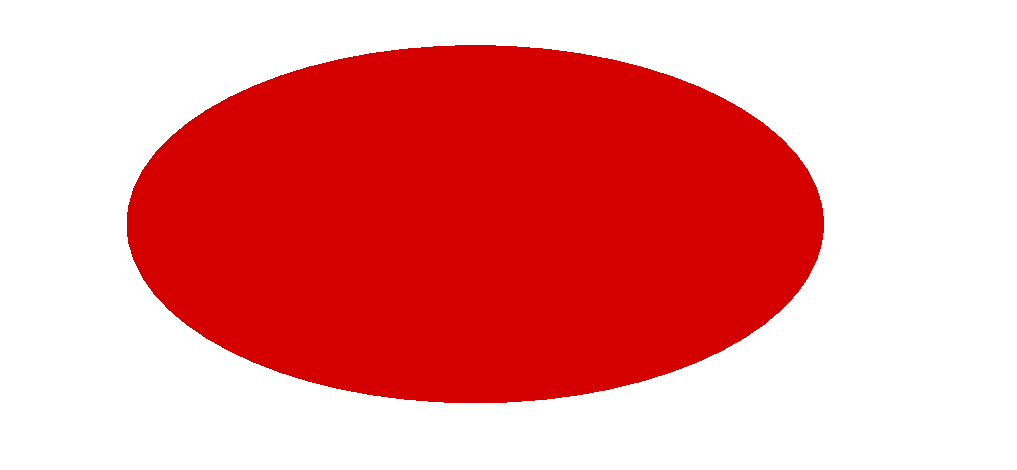
\includegraphics[width=\textwidth]{./img/todo}}	
			\caption{Kolekce v MongoDB využité pro běh programu.}
			\label{fig:colections}
		\end{figure}
	
		\subsection{Proces ukládání dat}
			Do kolekce terms jsou výrazy ukládán ihned po tom, co je určeno, že jsou správným termem. \todo{Lépe popsat dle kodu}
			
			Kolekce messages je plněna teprve po té, co se vrátí odpověď z MS Azure. Celá zpráva je ve třídě \textit{LogListener} ukládána do formátu \textit{AuditLogMessage}. Ta kopíruje svým obsahem právě kolekci messages. \textit{AuditLogMessage} je vlastníkem metody \textit{toDBObject}, která obsah třídy vráti ve vhodném formátu pro uložení do MongoDB.
			
			\begin{figure}[htb]\centering
				\tmpframe{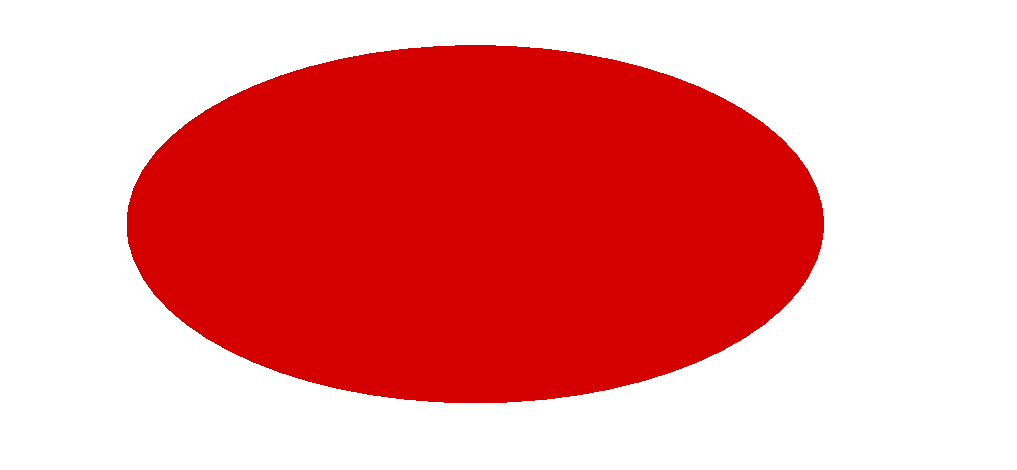
\includegraphics[width=\textwidth]{./img/todo}}	
				\caption{Sekvenční diagramy ukazující proces uložení dat do kolekcí terms a messages.}
				\label{fig:dataStoring-seq}
			\end{figure}
		
	\section{Napojení na Google Charts}
		Google vystavuje dokumentaci k produktu Google Charts na adrese \todo{Dodat adresu}. Samotné grafy jsou generovány pomoc javascriptu. Z knihovny grafů lze vybrat nepřeberné množství různorodých grafů. 
		
		\subsection{Rest API}
		Aby grafy byly generovány s daty z databáze bylo vytvořeno REST api. Toto api je postavené na míru Google Charts. Ovšem zpravidla není problém postavit další aplikaci tak, aby dokázala přijímat data z REST stejně popřípadě se je dokázala samostatně transformovat.
		
		Za tímto účelem vznikl kompletně celý modul aplikace. Tento modul má dovětek \textit{web-services}. Je složen ze dvou tříd:
		
		\begin{itemize} 
			\item DataProviderService
			\item ChartsProviderService			
		\end{itemize}
	
		Každá třída je chápana jako samostatná služba. 
		
		DataProviderService vystavuje webové služby na konkrétních URL adresách. Tím také poskytuje na jednotlivé GET \todo{Definovat zkratku GET} požadavky na zmíněné URL \todo{Definovat zkratku URL} odpovědi s daty z databáze. 
		
		Data z databáze ve správné struktuře vybíra služba promítnutá ve třídě ChartsProvderService.
		
		Jak bylo zmíněno, grafy z Google Charts očekávají konkrétní odpověď v předem určeném formátu JSON \todo{definovat JSON}. Ukázka projekce dat ve formátu JSON pro použití v grafu druhu Gauge \todo{Bud vlozit zdroj nebo url} je na obrázku \ref{fig:googleCharts-json}.
		
		\begin{figure}[htb]\centering
			\tmpframe{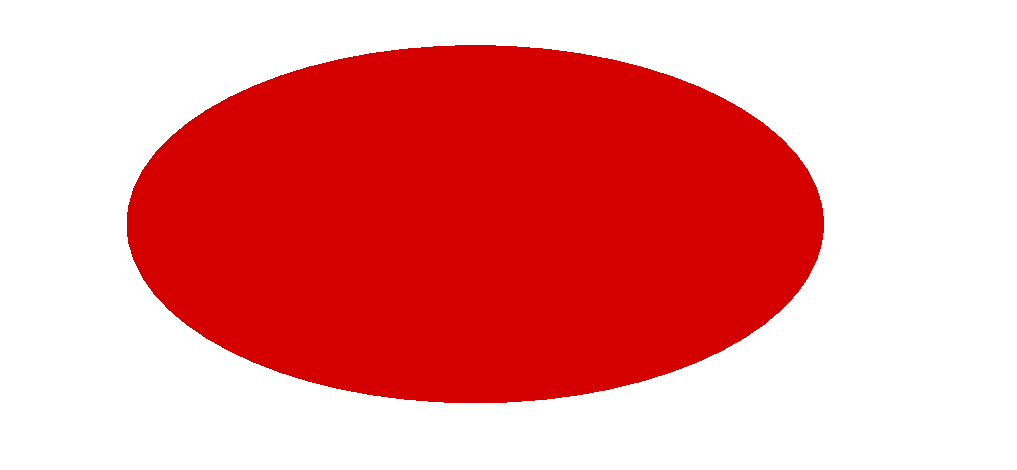
\includegraphics[width=\textwidth]{./img/todo}}	
			\caption{Data ve formátu json pro použití v Google Charts.}
			\label{fig:googleCharts-json}
		\end{figure}

\chapter{Analýza a vyhodnocení dat}
	\todo{Sem vepsat nějaký úvod k této kapitole}
	\blind[1]
	\todo{Popsat systém, na který to bylo nasazené}
	\blind[1]
	\section{Analýza K-Means}
		V této části je popsán celkový proces vytváření nejlepšího možného nastavení pro clusterovací k-means algoritmus. Jako základ jsem vybral trénovací data. U těchto dat jsem se rozhodl určit 1000 trénovacích vzorků. Protože cílem je detekovat bezpečnostní rizika a to jak ve formě špatných requestů tak i například podvržených zpráv, vybral z testovacích dat 500 vzorků, které dopadli chybou a 500 vzorků, které proběhli v pořádku. První množina slouží jako reprezentanti skupiny zpráv, které chceme rozpoznávat. Druhá množina 500 prvků je reprezentantem klasických zpráv, které by měli přes integrační platformu proudit.
		
		Pro poměr 50:50 jsem se rozhodl, aby byla dostatečně velká pravděpodobnost, že shluky v k-means najdou správná místa. Pokud bych zvolil poměr ve kterém by se podezřelé zprávy vyskytovali v malém množství nebo dokonce vůbec, algoritmus k-means by mohl pomocí shluků například rozpoznávat jednotlivé služby nebo najít zcela jiné vzory v datech. Takové vzory by se nemuseli hodit pro analýzu bezpečnostních rizik.
		
		Trénovací data jsem rozdělil náhodně poměrem 80:20 na trénovací a testovací. Testovací budou použita k odhadu správnosti shlukování. Vzhledem k tomu, že jsem jednoznačný identifikátor podezřelých zpráv označil, je možné na první pohled dokázat odlišit takovou zprávu od zprávy korektní.
		
		Následující sekce se zabívají jednotlivýma možnostma, jak ovlivnit běh algoritmu k-means. Pro všechny sekce byla použita stejná vstupní data.
		
		\todo{Když vznikne prosto, mohl by se vyzkoušet nějaký reálnější poměr.}

		\subsection{Počet shluků}
			K-means shlukuje data do $k$ shluků vhledem k podobnosti jednotlivých dat. V experimentu bezpečnostních rizik lze očekávat, že by rozdělení mohlo být na dvě skupiny:
			
			\begin{itemize} 
				\item data v pořádku
				\item podezřelá data		
			\end{itemize}
		
			I přes tuto myšlenku byl proveden experiment na různá množství shluků. Konkrétně na 2, 3, 4, 10 a 20. Všechny experimenty byly spuštěny současně na totožných vstupních datech. Hodnoty ostatních konfiguračních parametrů (samozřejmě mimo počtu shluků) byly zvoleny následující:
			
			\begin{itemize} 
				\item \textbf{výběr prvotních středových bodů: } náhodný
				\item \textbf{metrika: } eukleidova vzdálenost
				\item \textbf{počet běhů: } 100		
			\end{itemize}
		
				Výsledky jsou hromadně ilustrovány na obrázku \ref{fig:k-means-training}. Na ose x vždy pozorujeme shluky označené přirozeným číslem. Osa y zaznamená počet zpráv ve shluku.
				
				\subsubsection{2 shluky}
				
				Pro volby dvou shluků vznikly dva na počet zpráv téměr shodné shluky. Protože poměr vstupních dat 50:50 jde očekávaný výsledek \todo{očekávaný?}. Při kontrole konečných přiřazení shluků jsem narazil na zprávu, která by měla být označená jako podezřelá, ale bylo vyhodnocena jako zpráva korektní. V celé množině šlo o jedinou zprávu. Tato zpráva oznamovala, že došlo ke špatnému zadání hesla k jedné ze služeb. Jiná chyba nebyla nalezena \todo{asi ne uplne nazyvat chybou}. Lze tedy říci, že dochází k rozdělení na podezřelé zprávy a zprávy korektní. \todo{zkusit shrnout proč vznikla chyba}
				
				\subsubsection{3 shluky}
				Vizualizace výsledků přiřazení clusterů pro $k = 3$ nám ukazuje, že tři vzniklé shluky jsou o velikostech 35, 409 a 355 vzorků. Zde je rozdělení shluků takové, že jeden obsahuje pouze zprávy podezřelé. Další shluk obsahuje pouze zprávy v pořádku a stejně jako v případě dvou shluků podezřelou zprávu o špatném zadání hesla. Poslední, nejmenší shluk je kombinací. Po detailnějším rozboru vyplynulo, že zprávy v tomto shluku jsou oproti ostatním zprávám kratší. Normalizovaná zpráva se skláda zpravidla z několika slov. Výsledkem rozdělení trénovací množiny byly shluky podezřelých zpráv, korektních zpráv a velmi krátkých zpráv.
				
				\begin{figure}[htb]\centering
					\tmpframe{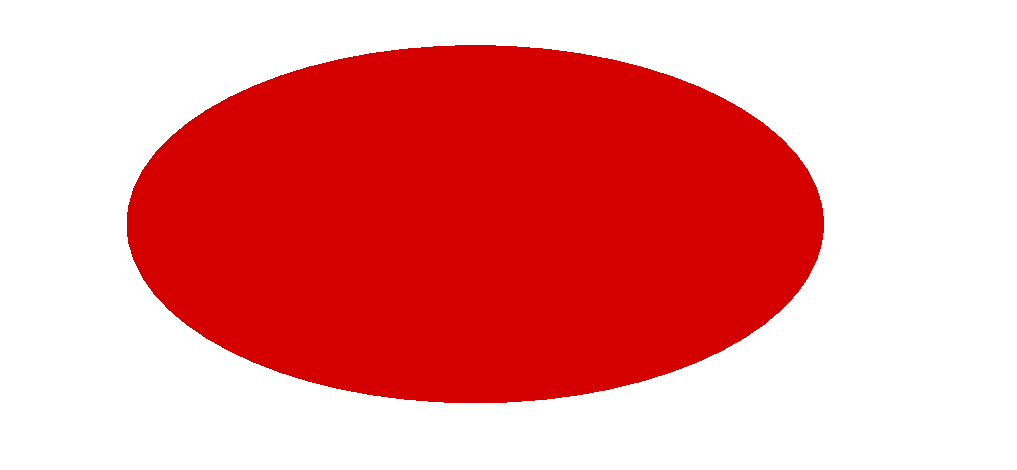
\includegraphics[width=\textwidth]{./img/todo}}	
					\caption{Zobrazené grafy s počtem zpráv v jednotlivých shlucích.}
					\label{fig:k-means-training}
				\end{figure}
				
				\subsubsection{4 shluky}
				Čtyři shluky ukázaly pro jejich velikost podobný výsledek jako když $k = 3$. Největší cluster obsahuje zprávy většinu korektních zpráv a již zmiňované krátké chybové zprávy. Druhý shluk obsahuje pouze chyby. Charakteristikou jde spíše o kratší zprávy převážně způsobené komponentou notifikačního enginu. Dále je přítomen shluk, jehož obsahem jsou jen zprávy chybové. Převážně jde o zprávy, které jsou delší a nesou například informaci o tom proč chyba nastala, nikoli pouze upozornění, že nastala. Poslední, obsahově nejmenší, shluk obsahuje pouze několik málo korektních požadavků. 
				
				\subsubsection{10 shluků}
				Experiment s deseti shluky ukazuje na trend, kdy se k-means přizpůsobuje jednotlivým službám. U dvou shluků došlo ke kolizi korektních a podezřelých požadavků. Oba tyto clustery shlukovali převážně kratší zprávy. U těch je větší pravděpodobnost, že jejich vektor bude převážně nulový. Ostatní shluky obsahují buď chyby nebo správné požadavky, jen se přizpůsobují ke konkrétním službám. Je zde možné například rozpoznávat shluk, který obsahuje chyby hlásící špatný KMS \todo{zkratka KMS} překlad a stejně tak shluk s chybami špatného přihlášení.
				
				\subsubsection{20 shluků}
				K-means s $k = 20$ potvrzuje vývoj, který se udál již při $k = 10$. Pouze jeden shluk je ze smíšených korektních zpráv a z podezřelých. Ten obsahuje pouze jeden záznam z podezřelých. Jednotlivé clustery více rozpoznávají jednotlivé služby a chyby. U chyb, jejichž druhů je ve vstupních dat méně než služeb se to projevuje více.
				
				\subsubsection{Shrnutí}
				Z celého vývoje dat, která byla použita na testování, plyne, že nejlepším je nechat dva shluky. Tím dokážeme rozlišit podezřelé zprávy od korektních. To zcela naplňuje požadavky detekce bezpečnostních rizik. Další možností je vytvořit shluků více a pokusit se i detekovat různé druhy chyb. Při této volbě bude vyžadováno více starostí organizováním, které clustery patří do jaké skupiny. Při velkém počtu shluků by mohlo docházet k přeučení, kdy by sice byly rozpoznávany konkrétní chyby konkrétní služby, ovšem s dalším nasazením nové služby by byly potíže.
		
		\subsection{Metrika}
			Pro porovnání různých způsobů měření vzdálenosti jsem zvolil na MS Azure dostnou eucleidovu vzdálenost (\ref{sec:eukleid_distance}) a cosinovu vzdálenost (\ref{sec:cosine_distance}). Protože celá analýza ideálního počtu shluků byla založena na eucleidově vzdálenosti, další měření stačí provést už pouze na cosinově vzdálenosti.
			
			Pro následující výsledky platí, že velikosti shluků jsou průměrovány z 10 spuštení programu. Nastavení k-means je následovné:
			\begin{itemize} 
				\item \textbf{výběr prvotních středových bodů: } náhodný
				\item \textbf{metrika: } cosinova vzdálenost
				\item \textbf{počet běhů: } 100		
			\end{itemize}
		
			Při zkoumání výsledků se objevil jev, kdy některé zprávy nebyly přiřazený do žádného clusteru. Po hlubší analýze jsem zjistil, že jde o zprávy, které pochází z B2B brány. Tyto požadavky po normalizaci mají velikost nula. To vede k tomu, že jejich vektor je nulový. S takovým vektorem má cosinova vzdálenost problém. Nelze jej vypočítat, tak zpráva není označena žádným shlukem.
			
			Kromě těchto nulových dat dochází k falešně pozitivnímu označení některých výrazně menších zpráv jako bezpečnostní rizika. Konkrétně pro případ, kde $k = 3$ došlo rozdělení dat žádného shluku (prázndé zprávy), podezřelé zprávy, korektní a další skupinu korektních. V této skupině dominovali zprávy z REST rozhraních. Ty se od ostatních požadavků liší, že nejsou v XML zápisu ale v JSON.
			
			Při náhledu, jak byly zprávy rozděleny do clusterů, při 4 shlucích lze opět pozorovat, že podezřelé zprávy jsou všechny z testovacích dat zahrnuty v jednom shluku. Ostatní shluky jsou složeny už pouze ze zpráv z běžné komunikace. Jejich rozdělení je pak závislé na charakteru zprávy.
			
			Deset shluků také vykazuje dokonalé rozdělení testovacích na rizika a ostatní zprávy. Obě skupiny jsou rozloženy do stejného počtu shluků.
			
			V případě $ k = 20$ jsou data opět rozdělena. Ovšem narozdíl od testovaných $k < 20$ se zde objevují clustery, které obsahují například jen jednu zprávu. 
			
			Z výsledků analýzy, kdy porovnáváme metriku euikleidovu a cosinovu je pozorovatelná lepší přesnost u cosinovy délky. Problém zde nastává se zprávy, které mají nulový vektor. Tyto zprávy je třeba ošetřit nebo nahradit normalizační funkci tak, aby nulový vektor negenerovala. 			
			
		\subsection{Inicializace}
			Vliv na běh algoritmu má i počáteční nastavení středů jednotlivých shluků. MS Azure ve svém modulu pro k-means nabízí možnosti \cite{MSAzure-kmeans}:
			
			\begin{itemize} 
				\item \textbf{Prvních N}. $N \in \mathbb{N} $ prvních vzorků z dat je určeno jako střed shluku. 
				\item \textbf{Náhodné}. Jsou vybrány náhodné body ze vstupních vzorků jako středy.
				\item \textbf{K-Means++}. Algoritmus definovaná Davidem Arthurem a Sergeiem Vassilvitskii \cite{kmeans++}
				\item \textbf{K-Means++Fast}. Optimalizovaná verze K-Means++.	
				\item \textbf{Rovnoměrně}. Středy jsou rozmístěné ve stejné vzdálenosti v prostoru.		
				\item \textbf{Dle popisku sloupce}. Algoritmus, který na základě popisu sloupe dat rozhoduje o tom, jak budou středy umístěny.			
			\end{itemize}
		
		Z experimentu jsem se rozhodl vyřadit K-Means++Fast, jenž je optimalizovanou verzí K-Means++ a inicializaci dle popisku sloupce, neboť jsem nedohledal oficiální dokumentaci k metodě, jak funguje.
		
		Pro experiment jsem zvolil následující nastavení:
		\begin{itemize} 
			\item \textbf{výběr prvotních středových bodů: } výběr pomocí komponenty Sweep K-means \todo{Přidat sweep k-means do volby počtu shluků.}
			\item \textbf{výběr prvotních středových bodů: } předmětem experimentu
			\item \textbf{metrika: } eukleidova i cosinova vzdálenost
			\item \textbf{počet běhů: } 100		
		\end{itemize}
	
		\todo{kmeans++ U kosinu 1 FP, ale ve skutecnosti slo o chybu, ze dms nenasla soubor!}
		\todo{PrvníchN eukl - 30 shluku}
		\todo{PrvníchN cosi - 30 shluku}
		\todo{Náhod. e - 11}
		\todo{Náhod. c - 12}
		\todo{even. e - 11}
		\todo{even. c - 22}
		
		Výsledky experimentu ukazuje tabulka \ref{tab:clustering_errors}. V tabulce se vyskytují počty zpráv, které byly v jednotlivých metodách označeny falešně pozitivní (dobrá zpráva označená jako podezřelá) a falešně negativní (podezřelá zpráva označená jako korektní). U všech běhů pro cosinovu metriku bylo 20 vždy 20 zpráv neoznačeno žádným číslem shluku. Jde o nulové vektory, které cosinova vzdálenost nedokáže vypočítat.
		
		Z tabulky (\ref{tab:clustering_errors}) se jeví nejlepší metoda prvních N. Porovnáme-li výsledky této tabulky s obrázkem \ref{fig:k-means-num-clusters}, který ukazuje graf závislosti počtu shluků na konkrétní metodě inicializace (výpočítané pomocí metody sweep clustering) je vidět, že metoda prvních vytváří velký počet shluků. Maximální počet byl stanoven na 30. Až na této hranici se prvních N zastavila. Vzniklo tím mnoho méně obsazených shluků. Jednotlivé zprávy byly rozděleny korektně na podezřelé a nepodezřelé. Velká počet shluků pak vedl i k většímu počtu rozeznaných chyb. Problém by mohl nastat s novou, v trénovacích datech neexistující, chybou. Proto i přes skvělý výsledek neshledávám tuto metodu ideální.
		
		Ve všech ostatních metodách inicializace se při měření eukleidovou metrikou objevila jedna stejná podezřelá zpráva, která byla označena jako nepodezřelá. Jde o chybu, která se svého druhu v trénovacích datech objevuje jediná. Celkově to ukazuje na slabost při zjišťování nových chyb.
		
		Cosinova metrika si vedla značně lépe, než eukleidova. Ve vstupních datech měla jen jeden případ špatného určení. Šlo o případ, kdy korektní zpráva byla označená za chybnou. Při bližším zkoumání jsem zjistil, že jde zprávu, která hlásí nenalezení dokumentu v uložišti. Ve skutečnosti algoritmus našel a označil jako chybu zprávu, která nesla informaci o chybě. Z pohledu administrátora platformu může jít o zajímavou informaci, neboť dotazuje-li se někdo na neexistující soubor jde také o bezpečnostní riziko.
		
		\begin{table}[htb]\centering
			\centering
			\caption{Zobrazení chyb při shlukování 800 vzorků, při rovnoměrném rozdělení korektních a podezřelých zpráv.}
			\label{tab:clustering_errors}
			\begin{tabular}{|l|llllllll}
				\hline
				\multirow{2}{*}{}  & \multicolumn{2}{l|}{Prvních N}                    & \multicolumn{2}{l|}{Náhodné}                      & \multicolumn{2}{l|}{K-Means++}                    & \multicolumn{2}{l|}{Rovnoměrně}                   \\
				& \multicolumn{1}{l|}{FP} & \multicolumn{1}{l|}{FN} & \multicolumn{1}{l|}{FP} & \multicolumn{1}{l|}{FN} & \multicolumn{1}{l|}{FP} & \multicolumn{1}{l|}{FN} & \multicolumn{1}{l|}{FP} & \multicolumn{1}{l|}{FN} \\ \hline
				Eukleidova metrika & 0                       & 0                       & 0                       & 1                       & 0                       & 1                       & 0                       & 1                       \\ 
				Cosinova metrika   & 0                       & 0                       & 0                       & 0                       & 1                       & 0                       & 0                       & 0                       \\ 
			\end{tabular}
		\end{table}
	
		\begin{figure}[htb]\centering
			\tmpframe{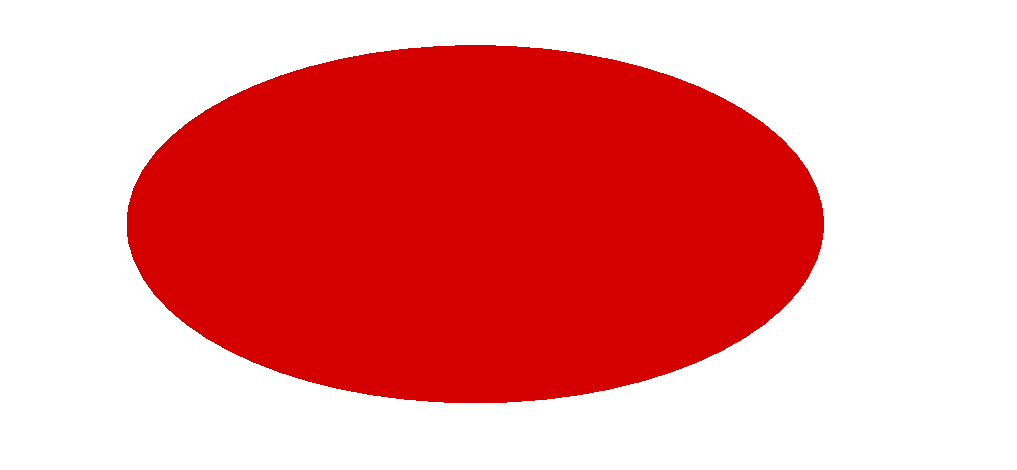
\includegraphics[width=\textwidth]{./img/todo}}	
			\caption{Počty clusterů, které jako ideální vyhodnotila metoda sweep k-means.}
			\label{fig:k-means-num-clusters}
		\end{figure}
	
		
	\section{Analýza detekce anomálie}
		\todo{Link do 2. kapitoly}
		Při detekci anomálie jsem kromě experimentů s ideálním nastavením vytvořil i experiment mezi dvěma metodami. Jedna je detekce anomálie založená na principu PCA, jejíž princip je přiblížen v kapitole \ref{sec:pca}. Druhou metodou je One-Class Support Vector Machine \todo{Udělat kapitolku.}, dále bude označována zkratkou SVM.
	
		\subsection{Popis vstupních dat}
		Rozdíl v přístupu mezi shlukováním a detekce anomálie je v trénovacích datech. Při detekování anomálií byla jako testovací data použita pouze data, která byla manuálně určena jako nezávadná. Dále byla připravena i množina dat testovacích. Testovací data obsahují v poměru 87:13 korektní zprávy a podezřelé.
		
		Velikost obou množin je 1000 požadavků. Vstupy byly vybrány náhodným výběrem z téměř 50000 požadavků velké množiny na ESB. Zprávy, které integrační platformou v pořádku prošli byly hodnoceny jako korektní. Zprávy, které vyvolávali chyby byly označené jako podezřelé. Nevýhodou tohoto přístupu může být přehlédnutí rizikové zprávy, která běžným pohledem se může jevit v pořádku.
		
		\subsection{Velikost vstupního vektoru}
			Při detekci anomálií jsem se jako jedním z konfiguračních parametrů zabýval s velikostí vstupního vektoru. Vliv, který má velikost vektoru byl zkoumán vždy pro ohodnocení klasifikace metodou \textit{Přesnost} (více v kapitole \ref{subsec:classification_performance}). Zkoumány byly metody detekce anomálie s využitím PCA a metoda s využitím SVM.
		
		\subsection{Ohodnocení klasifikace}
			\label{subsec:classification_performance}
			Pro dosažení nejlepšího možného výsledku používám MS Azure komponentu nazvanou \uv{Tune Model Hyperparameters.} Jde o komponentu, která se snaží optimalizovat parametry modelu, tak aby našla ideální nastavení \cite{msAzure}. Na základě toho je nutné být schopen rozeznat, jestli předchozí ohodnocení parametrů je horší než stávající. K tomu poslouží tyto možnosti nastavení \cite{powers-precision}:
			
			\begin{itemize} 
				\item \textbf{Přesnost: }  lze vyjádřit vzorcem $\frac{tp+tn}{tp+tn+fp+fn}$
				\item \textbf{Správnost: } lze vyjádřit vzorcem $\frac{tp}{tp+fp}$
				\item \textbf{Podíl: } lze vyjádřit vzorcem $\frac{tp}{tp+fn}$
				\item \textbf{F-score: } \todo{todo powers-precision}				
			\end{itemize}
		
			Experiment s ohodnocením klasifikace na základě přesnosti je zobrazen v tabulce \ref{table:anomaly_accuracy}. Lze pozorovat, že ani při jedné z použitých metod nedošlo k označení podezřelé zprávy ve zprávu korektní. Z hlediska bezpečnosti je lepší prověřovat správné zprávy, než ignorovat podezřelé. Jediný rozdíl je v tom, že SVM hodnotí méně korektních zpráv jako podezřelé. Při bližším pohledu na takové zprávy jde převážně o kratší požadavky.
			
			\begin{table}[htb]\centering
				\centering
				\caption{My caption}
				\label{table:anomaly_accuracy}
				\begin{tabular}{|l|l|l|l|l|}
					\hline
					\multirow{2}{*}{} & \multicolumn{2}{l|}{PCA}                 & \multicolumn{2}{l|}{SVM}                 \\ 
					& P-M: korektní & P-M: podezřelé & P-M: korektní & P-M: podezřelé \\ \hline
					Korektní          & 525                & 165                 & 656                & 34                  \\ \hline
					Podezřelé         & 0                  & 102                 & 0                  & 102                 \\ \hline
				\end{tabular}
			\end{table}
		
			Po změně hodnotícího vzorce na Správnost se výsledná data příliš nezměnila. V tabulce \ref{table:anomaly_precision} je vidět, že hodnoty pro SVM zůstali totožné, jako v případě použití Přesnosti. U PCA došlo k lehkému zhoršení. Toto zhoršení je rovno 14 korektním zprávám, které byly označené jako podezřelé.
		
			\begin{table}[htb]\centering
				\centering
				\caption{My caption}
				\label{table:anomaly_precision}
				\begin{tabular}{|l|l|l|l|l|}
					\hline
					\multirow{2}{*}{} & \multicolumn{2}{l|}{PCA}                 & \multicolumn{2}{l|}{SVM}                 \\ 
					& P-M: korektní & P-M: podezřelé & P-M: korektní & P-M: podezřelé \\ \hline
					Korektní          & 511                & 179                 & 656                & 34                  \\ \hline
					Podezřelé         & 0                  & 102                 & 0                  & 102                 \\ \hline
				\end{tabular}
			\end{table}
		
			Změna hodnocení na Podíl pro výsledek příliš změnu neznamenal (hlavně v porovnání s hodnocením Správnost). Tabulka \ref{table:anomaly_recall} ukazuje, že jediná změna oproti hodnocení Správnost je o jednu zprávu víc, která byla chybně označena jako podezřelá v případě použití PCA. SVM si stejně jako v předchozích dvou experimentech drží stejné hodnoty.
			
			\begin{table}[htb]\centering
				\centering
				\caption{My caption}
				\label{table:anomaly_recall}
				\begin{tabular}{|l|l|l|l|l|}
					\hline
					\multirow{2}{*}{} & \multicolumn{2}{l|}{PCA}                 & \multicolumn{2}{l|}{SVM}                 \\ 
					& P-M: korektní & P-M: podezřelé & P-M: korektní & P-M: podezřelé \\ \hline
					Korektní          & 510                & 180                 & 656                & 34                  \\ \hline
					Podezřelé         & 0                  & 102                 & 0                  & 102                 \\ \hline
				\end{tabular}
			\end{table}
		
			Použití F-Score vedlo k totožným výsledkům jako experiment s Přesností. Více ji znázorněno v tabulce \ref{table:anomaly_f-score}
		
			\begin{table}[htb]\centering
				\centering
				\caption{My caption}
				\label{table:anomaly_f-score}
				\begin{tabular}{|l|l|l|l|l|}
					\hline
					\multirow{2}{*}{} & \multicolumn{2}{l|}{PCA}                 & \multicolumn{2}{l|}{SVM}                 \\ 
					& P-M: korektní & P-M: podezřelé & P-M: korektní & P-M: podezřelé \\ \hline
					Korektní          & 525                & 165                 & 656                & 34                  \\ \hline
					Podezřelé         & 0                  & 102                 & 0                  & 102                 \\ \hline
				\end{tabular}
			\end{table}
		
			Při porovnání výsledků klasifikace F-Score a Přesnosti došlo ke zcela totožným výsledkům. Obě tyto metody byly z výše uvedených i nejvýše úspěšné z pohledu PCA. SVM nezaznamenalo žádnou změnu na hodnocení klasifikace.
		
			
	
		\todo{Popsat vstupní parametry}
		\todo{Ukázat výsledky na Prod logu}	
		\todo{Dojít k závěru}						
	
\chapter{Závěr}

\setsecnumdepth{part}
\chapter{Conclusion}


\bibliographystyle{iso690}
\bibliography{bibliography}

\setsecnumdepth{all}
\appendix

\chapter{Acronyms}
% \printglossaries
\begin{description}
	\item[GUI] Graphical user interface
	\item[XML] Extensible markup language
\end{description}


\chapter{Contents of enclosed CD}

%change appropriately

\begin{figure}
	\dirtree{%
		.1 readme.txt\DTcomment{the file with CD contents description}.
		.1 exe\DTcomment{the directory with executables}.
		.1 src\DTcomment{the directory of source codes}.
		.2 wbdcm\DTcomment{implementation sources}.
		.2 thesis\DTcomment{the directory of \LaTeX{} source codes of the thesis}.
		.1 text\DTcomment{the thesis text directory}.
		.2 thesis.pdf\DTcomment{the thesis text in PDF format}.
		.2 thesis.ps\DTcomment{the thesis text in PS format}.
	}
\end{figure}

\end{document}
